\documentclass[10pt]{article}

% Official TMLR style file (github.com/JmlrOrg/tmlr-style-file). Anonymous by default: do NOT add the
% [accepted] or [preprint] option for a submission -- non-anonymous submissions are rejected without review.
% The non-anonymous build is produced from main_preprint.tex, which passes [preprint].
\usepackage{tmlr}

\usepackage[T1]{fontenc}
\usepackage{microtype}
\usepackage{amsmath,amssymb}
\usepackage{booktabs}
\usepackage{enumitem}
\usepackage{multirow}
\usepackage{array}
\usepackage{graphicx}
\usepackage{xcolor}
\usepackage{tikz}
\usepackage{pgfplots}
\usetikzlibrary{arrows.meta,positioning,shapes.geometric,shapes.symbols,calc,fit,backgrounds,patterns,patterns.meta,decorations.pathreplacing}
\usepgfplotslibrary{groupplots}
\usepackage{hyperref}
\usepackage{url}
\usepackage{cleveref}

\hypersetup{colorlinks=true, linkcolor=black!70!blue, citecolor=black!70!blue, urlcolor=black!70!blue,
            pdftitle={Evidence-Basis Arbitration for Conflicting Persistent Memory in Small Tool-Using Agents},
            pdfsubject={Preregistered evaluation of gated enforcement for agent memory},
            pdfkeywords={LLM agents; persistent memory; memory conflict; evidence-basis arbitration;
                         selective enforcement; preregistration; reliability; harmful answers}}

% Shared visual language for every figure in the paper.
% Colours are from the Okabe--Ito colour-blind-safe set, chosen so that they also separate by lightness when the
% paper is printed in greyscale. Each experimental condition keeps the same colour in every figure.

% --- condition families -------------------------------------------------------------------------------------
\definecolor{cNone}{HTML}{6E6E6E}   % B      : memory, no labels                       (grey,        L* ~ 47)
\definecolor{cAdv}{HTML}{56B4E9}    % G, T   : advisory labels                         (sky blue,    L* ~ 72)
\definecolor{cEnf}{HTML}{D55E00}    % R, RT  : enforced record/temporal labels         (vermillion,  L* ~ 51)
\definecolor{cLLM}{HTML}{CC79A7}    % LA, LG : LLM arbiter                             (purple,      L* ~ 61)
\definecolor{cEvarb}{HTML}{009E73}  % EB and EBG variants: evidence-basis              (green,       L* ~ 57)
\definecolor{cEBG}{HTML}{00634A}    % EBG    : the full proposed mechanism             (dark green,  L* ~ 36)
\definecolor{cAll}{HTML}{E69F00}    % EBG-all: ungated enforcement, the counter-result (amber,       L* ~ 71)

% --- measurement roles --------------------------------------------------------------------------------------
\definecolor{cAcc}{HTML}{0072B2}    % accuracy / task success
\definecolor{cHarm}{HTML}{D55E00}   % harmful answers
\definecolor{cAbst}{HTML}{56B4E9}   % abstention
\definecolor{cFmt}{HTML}{CC79A7}    % format failures
\definecolor{cNeutral}{HTML}{BFBFBF}

% --- diagram furniture --------------------------------------------------------------------------------------
\definecolor{cBoxFill}{HTML}{F4F6F8}
\definecolor{cBoxEdge}{HTML}{394A59}
\definecolor{cAccentFill}{HTML}{E4F2EC}
\definecolor{cWarnFill}{HTML}{FBEFE4}
\definecolor{cInk}{HTML}{1A2129}

\tikzset{
  node distance=5mm and 7mm,
  blk/.style   = {draw=cBoxEdge, fill=cBoxFill, rounded corners=1.6pt, line width=0.5pt,
                  align=center, inner sep=3.4pt, font=\footnotesize, text=cInk, minimum height=7.2mm},
  blkacc/.style= {blk, fill=cAccentFill, draw=cEBG},
  blkwarn/.style={blk, fill=cWarnFill, draw=cEnf},
  blkplain/.style={blk, fill=white},
  dec/.style   = {draw=cBoxEdge, fill=white, line width=0.5pt, align=center, inner sep=3pt,
                  font=\scriptsize, text=cInk, shape=diamond, aspect=2.6, inner xsep=1pt},
  store/.style = {draw=cBoxEdge, fill=white, line width=0.5pt, align=center, font=\footnotesize,
                  text=cInk, cylinder, shape border rotate=90, aspect=0.22, inner sep=3pt},
  lbl/.style   = {font=\scriptsize, text=cInk, inner sep=1.5pt},
  flow/.style  = {->, >=latex, draw=cBoxEdge, line width=0.5pt},
  flowacc/.style={flow, draw=cEBG, line width=0.7pt},
  flowwarn/.style={flow, draw=cEnf, dash pattern=on 2.4pt off 1.6pt},
  flowback/.style={flow, draw=cNone, dash pattern=on 1.2pt off 1.4pt},
  grp/.style   = {draw=cNeutral, rounded corners=2pt, line width=0.5pt, inner sep=4pt},
}

% Consistent pgfplots look
\pgfplotsset{
  compat=1.18,
  paperaxis/.style={
    tick align=outside, tick pos=left,
    axis line style={draw=cInk, line width=0.4pt},
    every axis label/.append style={font=\footnotesize, text=cInk},
    tick label style={font=\scriptsize, text=cInk},
    legend style={font=\scriptsize, draw=cNeutral, fill=white, fill opacity=0.92, text opacity=1,
                  rounded corners=1pt, inner sep=2pt},
    grid style={draw=cNeutral, line width=0.3pt},
    label style={font=\footnotesize},
    title style={font=\small\bfseries, text=cInk},
  },
}


\newcommand{\pp}{\,pp}
\newcommand{\ci}[2]{[#1,\,#2]}
\newcommand{\cond}[1]{\textsf{#1}}
% file paths that may break across lines (hyperref's \nolinkurl breaks at / and _)
\urlstyle{tt}
\newcommand{\srcfile}[1]{\nolinkurl{#1}}

\title{Evidence-Basis Arbitration for Conflicting Persistent Memory\\in Small Tool-Using Agents:\\
A Pre-registered Evaluation of Gated Enforcement}

% Authors are deliberately absent: the tmlr package hides them unless [accepted]/[preprint] is given.
% Author details for the camera-ready are kept in AUTHOR_INFORMATION.md, not in this file.
\author{\name Anonymous Authors \email anonymous \\ \addr Anonymous Institution}

\def\month{11}
\def\year{2026}
\def\openreview{\url{https://openreview.net/forum?id=XXXX}}

% Give TeX a little slack so that long verbatim paths in captions do not overflow the text block.
\emergencystretch=6em
\hyphenpenalty=500
\tolerance=1200

\begin{document}
\maketitle

\begin{abstract}
Agents with persistent memory must act on records that contradict one another. The usual remedy --- attach
reliability labels derived from record metadata and enforce them at the terminal action --- can make small models
worse rather than better, because the agent follows the label instead of the text. We ask whether arbitration that
reports the \emph{evidence basis} for each resolution, and enforces only resolutions that basis supports, improves
reliability, and whether enforcing resolutions indiscriminately increases harmful answers.

We evaluate Evarb-0.2, a deterministic arbiter that assigns every record in a group a status, an explicit evidence
basis and a strength, shows those labels to the agent, and at the terminal action issues at most one reversible
notice while enforcing only strong-strength resolutions. Mechanism, analysis and hypotheses were frozen and
pre-registered before the confirmatory data existed. The campaign ran 18 model $\times$ decoding cells over 12
conditions on 268 sealed tasks in 135 families --- 57{,}888 agent runs with no missing pair, duplicate or harness
error --- on four primary open-weight models from two families (3B--8B) and two secondary models, under
family-clustered sign-flip permutation inference with Holm correction.

All four pre-registered contrasts are supported. Gated evidence-basis arbitration raised task success over enforced
record-and-temporal labels by $17.1$\pp{} (95\% CI \ci{12.2}{22.1}, Holm-adjusted $p=4\times10^{-5}$), over advisory
temporal labels by $14.5$\pp, over an LLM arbiter under the same gated policy by $15.9$\pp, and over unlabelled
memory by $15.3$\pp. The harmful-answer rate fell from 22.6\% to 3.1\% and arbitrary picks from 252 runs to 13.
Ablations place most of the benefit in the labels themselves ($+11.8$\pp{} with no enforcement at all) rather than
in enforcement ($+6.0$\pp), and the development finding that metadata labels \emph{hurt} small agents replicates on
sealed data.

Two results qualify the contribution. Enforcing every arbitration rather than only strong ones scored $9.7$\pp{}
\emph{higher} than the gated mechanism while more than doubling harm and raising false resolution from 1.9\% to
12.9\%: gating trades accuracy for safety rather than dominating it. And the same gating machinery driven by an LLM
arbiter gave no success gain and $8.1$\pp{} more harm, indicating that enforcement inherits the reliability of
whatever supplies its labels. Effects also differ by model family: the Llama models gain by converting abstentions
into answers rather than harmful answers into correct ones. We report the pre-registered outcome, the exploratory
trade that cuts against our own design, and an unplanned mid-campaign platform transition affecting 1.69\% of rows
whose removal moves the pooled estimates by at most $0.1$\pp.

\end{abstract}

\vspace{-2mm}
\noindent\textbf{Keywords:} persistent memory for LLM agents; memory conflict resolution; evidence-basis
arbitration; selective enforcement; pre-registered evaluation; reliability and harmful answers; small open-weight
models.
\vspace{1mm}

\section{Introduction}
\label{sec:intro}

An agent with persistent memory is an agent that will eventually read two records that disagree. A budget was
revised, a deadline moved, a staging port changed; the store holds both the old statement and the new one, and
sometimes holds two statements that nothing in the record metadata can order. What the agent does at that moment
determines whether persistent memory is an asset or a liability.

The common engineering answer is to label records by reliability --- derived from when each was written --- and to
enforce those labels at the terminal action, so that the agent cannot submit a value the labelling says is stale.
This paper reports that, for small open-weight agents, both halves of that answer can misfire, and measures by how
much.

\subsection{Two failures that motivate the work}

The study began from a specific failure observed during development, not from a general belief that memory
safeguards help. In an exploratory pilot on development splits we gave small agents reliability labels derived only
from record metadata --- the date a record was written. When that metadata could not order the records, as for a
same-day correction or a pair ordered only by dates stated in the text, the labels declared the records
``conflicting''. The agents followed the label instead of the text. For one 7B model on same-day corrections,
correct runs fell from 22 of 24 without labels to 3 of 24 with metadata labels. Enforcing the labels at the terminal
action did not repair this, because enforcement reads the same labels.

A follow-up arbiter that ordered records from textual evidence removed much of that harm on held-out development
phrasings, but exposed the counterpart risk. When the arbiter itself resolved a genuine conflict wrongly --- a
negated cue read as a correction --- enforcement turned five or six of six correct \cond{conflict} answers per model
into arbitrary picks. We call this \textbf{false-resolution harm}: a mechanism confidently asserts an ordering the
evidence does not support, and the agent, or the harness acting for it, commits to a wrong value.

These two failures have the same shape. A reliability signal is produced from the wrong information, and the
machinery downstream --- the agent's deference, or the policy's enforcement --- amplifies it.

\subsection{Approach}

We test \textbf{evidence-basis arbitration}. A deterministic arbiter, Evarb-0.2, assigns every record in a group of
same-attribute records a status together with the \emph{evidence basis} for that status --- an explicit correction
naming the rival value, a stated validity date, the record date, an authoritative source, a genuine contradiction,
or insufficient evidence --- and a \emph{strength}: strong, moderate or none. The agent is shown these labels. At the
terminal action a policy may send one reversible notice when the submitted answer disagrees with the arbitration,
but it \emph{enforces} only resolutions of strong strength. This is \textbf{gating}. If the agent's response to a
notice is unusable, the pre-notice answer stands (\textbf{safe submission}). The full condition, \cond{EBG}, also
asks the agent to search memory before submitting when it has not done so.

The central question has two halves, and we test both:

\begin{quote}
Does evidence-basis-aware arbitration improve persistent-memory reliability in tool-using LLM agents, and can
indiscriminate enforcement of memory labels cause more harmful answers despite improving raw accuracy?
\end{quote}

\subsection{Contributions}

\begin{table}[h]
\centering
\caption{What this paper contributes, and where each claim is supported. ``Confirmatory'' means pre-registered and
frozen before the data existed; everything else is labelled as it is reported.}
\label{tab:contributions}
\small
\begin{tabular}{@{}p{0.46\linewidth}p{0.26\linewidth}p{0.22\linewidth}@{}}
\toprule
\textbf{Contribution} & \textbf{Status of the evidence} & \textbf{Where} \\
\midrule
A pre-registered confirmatory comparison of gated evidence-basis enforcement against enforced record-and-temporal
labels, advisory temporal labels, an LLM arbiter under the same policy, and unlabelled memory, with Holm
correction over the four contrasts.
& Confirmatory & \Cref{sec:results}, \Cref{fig:forest} \\[2pt]
A measurement of the cost of enforcing labels the evidence does not support: harmful-answer and false-resolution
rates per condition, including the pre-registered harm test.
& Confirmatory (harm test); descriptive rates & \Cref{sec:results}, \Cref{fig:tradeoff} \\[2pt]
Component ablations that separate labels, enforcement, gating, safe submission and search-before-submit --- and
show that gating \emph{costs} accuracy.
& Exploratory, BH-adjusted & \Cref{sec:ablations} \\[2pt]
A deterministic-versus-LLM arbiter comparison under one identical downstream policy, separating arbitration
quality from policy.
& Exploratory & \Cref{sec:ablations} \\[2pt]
A sealed evaluation set whose gold is fixed before any text exists, with blind model annotation; released with
hashes. We do not present it as a benchmark of record.
& Artifact & \Cref{sec:dataset} \\[2pt]
A pre-stated account of the mechanism's known failures, written before any confirmatory outcome, extended
afterwards without softening.
& Pre-registered, then extended & \Cref{sec:limitations} \\
\bottomrule
\end{tabular}
\end{table}


The mechanism was frozen before the confirmatory data set was built, and the analysis was pre-registered and frozen
before any confirmatory run. The campaign produced 57{,}888 agent runs with no missing pair, no duplicate and no
harness error.

\textbf{Results.} All four pre-registered contrasts are supported: \cond{EBG} raised task success over enforced
record-and-temporal labels by $17.1$\pp, over advisory temporal labels by $14.5$\pp, over an LLM arbiter under the
same gated policy by $15.9$\pp, and over unlabelled memory by $15.3$\pp, each with a bootstrap interval clear of
zero after Holm correction and in the same direction for all six models. The harmful-answer rate fell from 22.6\% to
3.1\% and arbitrary picks from 252 runs to 13.

\textbf{And two results that cut against the proposed design.} Enforcing every arbitration instead of only
strong-strength ones scored $9.7$\pp{} \emph{higher} while more than doubling harm; and the same gating driven by an
LLM arbiter gave no gain and $8.1$\pp{} more harm. We report these as prominently as the supportive results, because
together they locate the contribution more precisely than the headline contrasts do: what matters is not
enforcement, and not gating, but having an evidence basis that tells enforcement where to stop.

\subsection{Scope}

The study concerns small open-weight models (3B--14B) in one synthetic tool-use harness with templated records,
English text and ISO-format value dates. It makes no claim about frontier models, natural memory logs, implicit
conflicts without lexical cues, or other harnesses. \Cref{sec:limitations} lists the limitations that were fixed
before the confirmatory results existed, and those the results themselves revealed.

\section{Problem formulation}
\label{sec:problem}

\paragraph{Setting.} An agent answers a question about the current (or a historical) value of an attribute by
calling a memory-search tool and then submitting a final answer. The store contains a group of records about that
attribute, written at different times, some of which assert values that disagree. The agent's terminal action is
three-way: submit a value, submit \cond{conflict} when the evidence does not determine one, or abstain.

\paragraph{What a resolution mechanism must decide.} Given a group of records $R=\{r_1,\dots,r_k\}$ about one
attribute, a mechanism must produce, for each record, a status (established, superseded, historical, unresolved)
and --- this is the part we vary --- must decide what to \emph{do} with that status at the terminal action. Three
designs span the space we study:

\begin{description}[leftmargin=1.2em]
\item[Advisory.] The status is shown to the agent and nothing more. The agent may ignore it. Conditions
\cond{G} (metadata labels), \cond{T} (temporal labels), \cond{EB} (evidence-basis labels) and \cond{LA} (LLM
arbiter) are advisory.
\item[Ungated enforcement.] Every resolution the mechanism produces is enforced at the terminal action: a
submission that disagrees is blocked or corrected. Conditions \cond{R}, \cond{RT} and \cond{EBG-all} enforce
without discrimination.
\item[Gated enforcement.] Only resolutions whose evidence basis is strong enough are enforced; the rest are
advisory. Conditions \cond{EBG} (and its variants) and \cond{LG} are gated; they differ in \emph{who} produces the
resolutions.
\end{description}

\paragraph{Why the distinction matters.} A reliability label is itself an inference, and it can be wrong in two
ways that have opposite remedies. It can be \emph{under-determined} --- the metadata cannot order two records, so
the mechanism reports a conflict that the text would resolve --- and it can be \emph{over-determined} --- the
mechanism asserts an ordering the evidence does not support. Advisory labelling leaves both errors to the agent,
which for small models means they are often followed anyway. Ungated enforcement removes the agent's discretion,
which converts an over-determined label directly into a wrong committed answer. Gating is the proposal that a
mechanism should enforce only where it can say \emph{why} it is sure.

\paragraph{Outcomes.} The frozen scorer classifies each run as correct or into one of several failure categories.
Two matter throughout. An answer is \textbf{harmful} if it commits to a wrong value: \cond{wrong\_value},
\cond{stale\_value}, \cond{unsupported\_claim} or \cond{arbitrary\_pick}. A group that genuinely cannot be ordered
is \textbf{falsely resolved} if the agent asserts a value for it instead of reporting a conflict. Task success and
harm are reported separately throughout, because, as \Cref{sec:ablations} shows, they do not move together.

\paragraph{Unit of analysis.} The unit is the task. Success per task is the mean over a model's decodings; contrasts
are paired within model and decoding; the clustering unit is the task \emph{family}, a (category, attribute) pair.
This matters because tasks within a family share a template and are not independent.

\section{Related work}
\label{sec:related}

Our literature search covered arXiv and closed on 14 November 2026; most entries were read at abstract level, and
six were read in full. Statements of the form ``we found none'' should therefore be read as ``in the work we
examined''. Extending the search to non-arXiv venues and to later work is an open item
(\Cref{sec:limitations}).

\subsection{Memory architectures}

Persistent memory for language-model agents is normally a store outside the context window that the agent reads
through retrieval or tool calls. MemGPT manages memory tiers by analogy with an operating system
\citep{packer2023memgpt}; Mem0 extracts, consolidates and retrieves salient facts across sessions
\citep{chhikara2025mem0}; Zep organises memory as a temporal knowledge graph \citep{rasmussen2025zep}; MEMOIR adds
a training-free lifecycle with judge-gated consolidation \citep{anand2026memoir}. These are background: our harness
uses a deliberately simple store (hashed bag-of-words retrieval, top four) so that the object of study is what
happens \emph{after} retrieval.

\subsection{Staleness, conflict and resolution}

\paragraph{Resolution rather than retrieval.} DISCERN preserves an immutable event log at write time, derives a
bitemporal fact store, and at read time lets the agent navigate with deterministic, LLM-free tools; the committed
action is a decidable function of the graph, guarded by gates including an earned-abstain gate that rejects
abstaining without searching \citep{ahuja2026discern}. It reports recall and currency as near-saturated and
resolution as the unsolved part. Its backbones are large hosted models, its facts and validity intervals are
LLM-extracted, and its ablations do not perturb extraction or timestamps.

\paragraph{Provenance and invalidation.} PACMI propagates invalidation through a provenance graph with a four-state
validity lattice and corrects outdated premises advisorily, by adding old and current facts to the answer prompt
\citep{wang2026pacmi}. AMV-Guard treats re-verification of a memory premise before a state-changing action as a
value-of-information stopping problem \citep{wang2026amvguard}. Governed Persistent Memory uses a bitemporal
state-transition model with deterministic, fail-closed release \citep{xu2026gpm}. TOKI formalises contradiction
resolution as write-time concurrency control over bitemporal operators \citep{wang2026toki}; StateWise repairs
invalid stored state before agent actions \citep{peng2026statewise}; PPMF and MemLineage bind tool authority or
lineage to the source of a memory \citep{xu2026ppmf,ouyang2026memlineage}. \citet{zhao2026accept} observe that
outdated memory and poisoning call for opposite write decisions and propose an evidence-conditioned accuracy
metric; \citet{zhou2026manysteps} give a theory of when memory reuse is safe.

\paragraph{Benchmarks.} STALE provides 400 scenarios and 1{,}200 queries over three dimensions including state
resolution and premise resistance \citep{chao2026stale}; its construction deliberately excludes explicit
invalidation, so it contains none of the lexically signalled cases Evarb targets and is the natural external test
of what a lexical arbiter cannot do. MemoryAgentBench includes a conflict-resolution competency
\citep{hu2025memoryagentbench}, and \citet{pakhomov2026bookkeeping} show that a frozen last-write rule already
answers a large share of its conflict split. LongMemEval and LoCoMo evaluate long-term conversational memory
including knowledge updates and abstention \citep{wu2024longmemeval,maharana2024locomo}.

\paragraph{Why models fail on updates.} CICM studies in-context updates mechanistically: probes still recover the
updated value when the model answers with the old one, and compliance with an advisory reminder depends on the
model family \citep{guo2026cicm}. That is the closest prior evidence on whether small models follow advisory signals
about which value is current, although its setting is single-answer dialogue rather than an agent with a three-way
terminal action. \citet{xu2026delivered} find that delivered memory often does not change agent behaviour;
\citet{pathirage2026confident} study when models search beyond parametric memory; \citet{zhang2026horn} issue
deterministic answer/search/abstain decisions from sufficiency certificates.

\subsection{Verification and self-correction}

Same-model self-correction without external feedback often fails to improve reasoning and can degrade it
\citep{huang2023selfcorrect,kamoi2024survey}; retrieval-side critique and correction are studied in Self-RAG and
Corrective RAG \citep{asai2023selfrag,yan2024crag}. Our LLM-arbiter conditions (\cond{LA}, \cond{LG}) use the
agent's own model to arbitrate records. They are not self-correction of the answer, but their errors are of the same
kind: an unaided small model judging evidence.

\subsection{What is new, and what is not}
\label{sec:novelty}

We state the negative half first, because the positive claim is narrow.

\textbf{Not new, and not claimed.} That memory improves memory-dependent tasks. That provenance, bitemporal
ordering or deterministic gating improve staleness and conflict handling
\citep{ahuja2026discern,wang2026pacmi,xu2026gpm,wang2026toki} --- indeed a deterministic last-write rule already
does well on an existing conflict benchmark \citep{pakhomov2026bookkeeping}. Ordering by a stated validity date
before the record date, which is standard bitemporal practice \citep{jensen1999temporal}. Forcing a search before
abstaining, which is essentially DISCERN's earned-abstain gate. That same-model verification without an external
signal can hurt \citep{huang2023selfcorrect,kamoi2024survey}. That agents often fail to use delivered memory and can
bind a stale value while still encoding the update \citep{xu2026delivered,guo2026cicm}. And combining known
components into one system is not in itself a contribution.

\textbf{What may be defensible.} Among the work we examined we found none that

\begin{enumerate}[leftmargin=1.6em,itemsep=1pt,topsep=2pt]
\item \textbf{exposes the evidence basis and strength of each resolution to the agent and gates enforcement on that
strength}, so that an ordering inferred from record dates, or an unreferenced correction, is advised while an
explicit referenced correction is enforced --- the enforcing systems we read apply their gates uniformly over a
structure built at write time;
\item \textbf{measures, on the same small open-weight models, what happens to the answer when the reliability
structure is wrong} --- both the harm of following wrong labels and the harm of enforcing them;
\item \textbf{compares a deterministic arbiter and an LLM arbiter under an identical downstream policy} on agents of
3B--14B, so that arbitration quality and policy are separated.
\end{enumerate}

What we contribute is therefore not a temporal rule but a measurement: of label-induced and enforcement-induced
harm on small agents, and a pre-registered test of whether basis-gated enforcement reduces that harm without losing
the benefit of enforcement. \Cref{tab:related} places the six full-text papers against the design dimensions this
study varies.

\begin{table}[t]
\centering
\caption{The six closest systems we read in full, against the design dimensions this study varies. Entries for
prior work describe what those papers do, not how well they do it. The last column states what this study
\emph{tests}, not what it finds.}
\label{tab:related}
\scriptsize
\setlength{\tabcolsep}{3pt}
\begin{tabular}{@{}p{0.165\linewidth}p{0.10\linewidth}p{0.08\linewidth}p{0.10\linewidth}p{0.085\linewidth}p{0.095\linewidth}p{0.085\linewidth}p{0.14\linewidth}@{}}
\toprule
\textbf{Dimension} & \textbf{DISCERN} & \textbf{PACMI} & \textbf{AMV-Guard} & \textbf{GPM} & \textbf{STALE} & \textbf{CICM} & \textbf{This study} \\
\midrule
Who makes the terminal decision
 & det.\ code over an LLM-built graph & LLM, prompt-level correction & decision-theoretic gate
 & det.\ services & LLM, constrained readout & the model (reminder or steering)
 & the agent; policy may send one reversible notice \\[2pt]
Same information advisory vs enforced, compared
 & no & no & vs fixed policies & governed vs ungoverned & not directly & reminder vs routing
 & \textbf{yes} (\cond{T}/\cond{RT}; \cond{EB}/\cond{EBG}; \cond{LA}/\cond{LG}) \\[2pt]
Labels state their evidence basis; enforcement gated on it
 & no (uniform gates) & no & no & no & no & no
 & \textbf{tested} (\cond{EBG}/\cond{EBG-all}) \\[2pt]
Deterministic vs LLM arbiter under one policy
 & no & no & no & no & no & no & \textbf{tested} (\cond{EBG}/\cond{LG}) \\[2pt]
Agents $\le$ 14B, open weights
 & no & no & no & baseline only & partly & yes, not agentic & yes (3B--14B) \\[2pt]
Cost of a wrong reliability label measured
 & no & partly & modelled & fail-closed by design & implicit & no
 & harmful-answer rate per condition \\
\bottomrule
\end{tabular}
\end{table}


\section{Method: Evarb-0.2}
\label{sec:method}

% Figure 1 -- system architecture. Drawn from the implementation: memlab (harness, tools, scorer),
% evarb/{arbiter,policy,render,clients}.py, agentrun_v2.parser, scripts/run_p2.py.
% Explicit mm coordinates: nothing overlaps, nothing leaves the text block.
\begin{figure}[t]
\centering
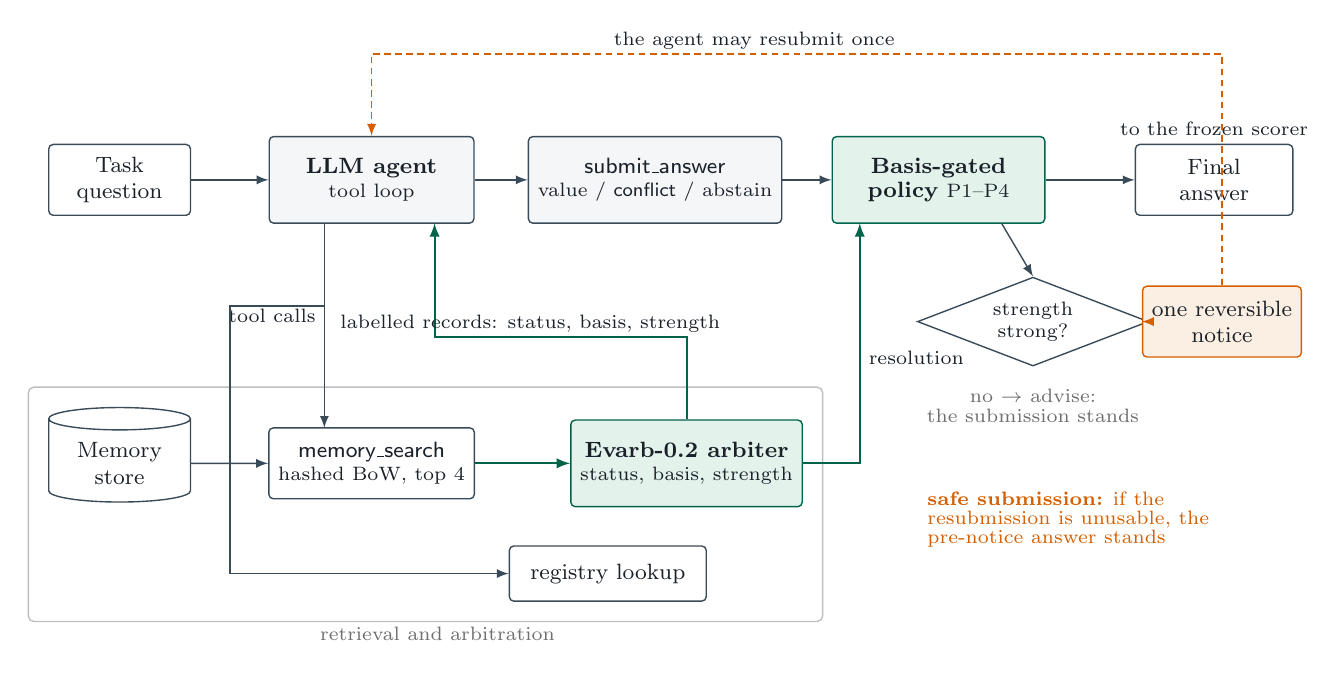
\begin{tikzpicture}[font=\footnotesize, x=1mm, y=1mm]

% ---------------- row A (y=46): the agent's control flow
\node[blkplain, minimum width=18mm, minimum height=9mm]  (task)   at (12,46) {Task\\question};
\node[blk,      minimum width=26mm, minimum height=11mm] (agent)  at (44,46) {\textbf{LLM agent}\\[-1pt]\scriptsize tool loop};
\node[blk,      minimum width=26mm, minimum height=11mm] (submit) at (80,46) {\cond{submit\_answer}\\[-1pt]\scriptsize value / \cond{conflict} / abstain};
\node[blkacc,   minimum width=27mm, minimum height=11mm] (policy) at (116,46) {\textbf{Basis-gated}\\[-1pt]\textbf{policy} \scriptsize P1--P4};
\node[blkplain, minimum width=20mm, minimum height=9mm]  (final)  at (151,46) {Final\\answer};

% ---------------- row B (y=28): the gate and the single notice
\node[dec, minimum width=16mm] (gate)   at (128,28) {strength\\strong?};
\node[blkwarn, minimum width=20mm, minimum height=9mm] (notice) at (152,28) {one reversible\\notice};

% ---------------- row C (y=10): retrieval and arbitration
\node[store,    minimum width=18mm, minimum height=12mm] (store) at (12,10) {Memory\\store};
\node[blkplain, minimum width=25mm, minimum height=9mm]  (retr)  at (44,10) {\cond{memory\_search}\\[-1pt]\scriptsize hashed BoW, top 4};
\node[blkacc,   minimum width=26mm, minimum height=11mm] (arb)   at (84,10) {\textbf{Evarb-0.2 arbiter}\\[-1pt]\scriptsize status, basis, strength};
\node[blkplain, minimum width=25mm, minimum height=7mm]  (reg)   at (74,-4) {registry lookup};

% ---------------- control flow
\draw[flow] (task) -- (agent);
\draw[flow] (agent) -- (submit);
\draw[flow] (submit) -- (policy);
\draw[flow] (policy) -- (final);
\node[lbl, above=0.4mm of final] {\scriptsize to the frozen scorer};

% ---------------- retrieval and arbitration
\draw[flow] (38,40.5) -- node[lbl, left, pos=0.45, xshift=-0.5mm] {\scriptsize tool calls} (38,14.5);
\draw[flow] (38,30) -- (26,30) -- (26,-4) -- (reg.west);
\draw[flow] (store) -- (retr);
\draw[flowacc] (retr) -- (arb);
\draw[flowacc] (arb.north) -- (84,26) -- node[lbl, above, pos=0.62]
      {\scriptsize labelled records: status, basis, strength} (52,26) -- (52,40.5);
\draw[flowacc] (arb.east) -| node[lbl, pos=0.72, right, xshift=0.5mm] {\scriptsize resolution} (106,40.5);

% ---------------- the gate
\draw[flow] (124,40.5) -- (gate.north);
\draw[flowwarn] (gate) -- (notice);

ode[lbl, text=cEnf, anchor=south] at (139,31.5) {\scriptsize yes};
\draw[flowwarn] (notice.north) -- (152,62) -- node[lbl, above, pos=0.55]
      {\scriptsize the agent may resubmit once} (44,62) -- (agent.north);
\node[lbl, text=cNone, align=center, anchor=north] at (128,20)
  {\scriptsize no $\rightarrow$ advise:\\[-1pt]\scriptsize the submission stands};

\node[lbl, text=cEnf, align=left, anchor=north west] at (114,7)
  {\scriptsize \textbf{safe submission:} if the\\[-1pt]\scriptsize resubmission is unusable, the\\[-1pt]\scriptsize pre-notice answer stands};

\begin{scope}[on background layer]
\node[grp, fit=(store)(retr)(arb)(reg), inner sep=2.5mm,
      label={[lbl, text=cNone, anchor=north west, xshift=1mm]below left:\scriptsize retrieval and arbitration}] {};
\end{scope}
\end{tikzpicture}

\vspace{1mm}
\caption[AGENTRUN / Evarb system architecture]{%
\textbf{System architecture.} Everything the study varies lives in the two shaded components. The
\emph{arbiter} decides what the agent is told about a group of records --- a status, the evidence basis for that
status, and a strength. The \emph{policy} decides what happens when the agent's submission disagrees with the
arbitration: it may send at most one reversible notice, and it enforces only when the resolution's strength passes
the gate. The store, the retrieval function, the tool schemas, the prompts and the scorer are identical in all
twelve conditions. Advisory conditions keep the arbiter and disable the policy; ungated conditions widen the gate
to accept moderate strength as well as strong.\\
\emph{Accessible description:} a left-to-right control flow along the top (task, agent, submission, policy, final
answer); a lower band in which the memory store feeds search and search feeds the arbiter, which both returns
labelled records to the agent and sends its resolution to the policy; below the policy a strength gate either
issues one notice, which returns to the agent along the top of the figure, or lets the submission stand.\\
\emph{Source:} drawn from the implementation (\texttt{memlab}, \texttt{evarb/\{arbiter,policy,render\}.py},
\srcfile{scripts/run_p2.py}); no component is hypothetical.}
\label{fig:architecture}
\end{figure}


\subsection{System architecture}

\Cref{fig:architecture} shows the harness. The agent is a local causal LM with a Hermes-style tool template. It
has three tools: \cond{memory\_search}, a hashed bag-of-words retrieval returning the top four records; a registry
lookup that may fail by design; and \cond{submit\_answer}, the terminal action, which takes a value, the literal
\cond{conflict}, or an abstention.

Between retrieval and the agent sits the \textbf{arbiter}, and between the agent's submission and the recorded
answer sits the \textbf{policy}. Everything we vary lives in those two places: the arbiter decides \emph{what the
agent is told} about the records, and the policy decides \emph{what happens} when the agent's submission disagrees
with that. The store, the retrieval function, the tool schemas, the prompts and the scorer are identical in all
twelve conditions.

\subsection{Arbitration}

The arbiter receives the records of one (entity, attribute) group. Each record has an identifier, a value, a text,
a source and a possibly-missing \cond{recorded\_on} date. It returns a resolution kind (\cond{unchallenged},
\cond{resolved}, \cond{contradiction}, \cond{unresolved}), an \emph{evidence basis}, a \emph{strength}
(\cond{strong}, \cond{moderate}, \cond{none}), the current value if any, and a per-record status.

\paragraph{Clause-level cues.} Each record text is split into clauses at sentence ends, semicolons and dashes.
Within a clause the arbiter looks for cues of seven kinds --- correction, supersession, dismissal, retention,
unconfirmed, contradiction, and a hypothetical value --- and qualifies each by its scope: \emph{negated} if a
negator occurs among the four tokens before the cue; \emph{quoted} if the cue is in quotation marks or the clause
contains a reporting verb; \emph{hypothetical} if the clause contains a conditional or modal marker. A clause
\emph{refers to a rival record} if it mentions the rival's value (token-bounded, numbers compared numerically) or
uses an anaphor for an earlier value when exactly one rival value exists. Validity dates are read after ``as of'',
``effective'', ``valid from'', ``since'' and similar phrases; a date equal to the record's own value is never
treated as a validity date.

\paragraph{Evidence bases.} Every resolution carries one of ten evidence bases, and strength is a function of the
basis and its conditions (\Cref{fig:bases}). The scope qualifiers are what separate this from a lexical rule
list: a correction cue inside a negated, quoted or hypothetical clause does not license the ordering that the same
cue would license when asserted.

% Figure 2 -- the arbitration workflow, in the order implemented by evarb/arbiter.py (arbitrate()).
% All content is kept inside x in [8,148] so the picture sits squarely in the text block.
\begin{figure}[t]
\centering
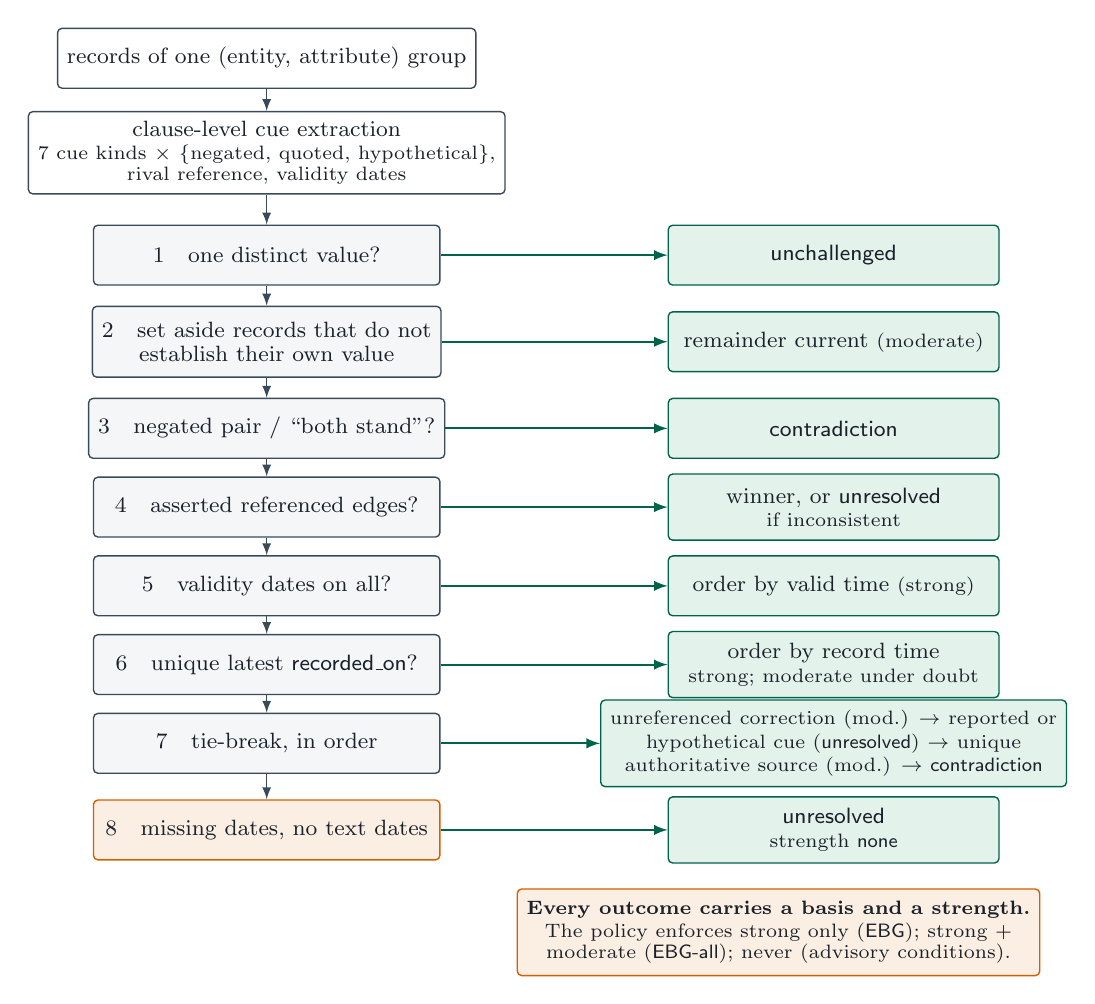
\begin{tikzpicture}[font=\footnotesize, x=1mm, y=1mm,
  wfstep/.style={blk, minimum width=44mm, minimum height=7.6mm},
  wfout/.style={blkacc, minimum width=42mm, minimum height=7.6mm}]

\node[blkplain, minimum width=44mm, minimum height=7.6mm] (in) at (36,92)
  {records of one (entity, attribute) group};
\node[blkplain, minimum width=56mm, minimum height=9mm] (clause) at (36,80)
  {clause-level cue extraction\\[-1pt]\scriptsize 7 cue kinds $\times$ \{negated, quoted, hypothetical\},\\[-2pt]\scriptsize rival reference, validity dates};

\node[wfstep] (s1) at (36,67) {1\quad one distinct value?};
\node[wfstep, minimum height=9mm] (s2) at (36,56) {2\quad set aside records that do not\\[-1pt]establish their own value};
\node[wfstep] (s3) at (36,45) {3\quad negated pair / ``both stand''?};
\node[wfstep] (s4) at (36,35) {4\quad asserted referenced edges?};
\node[wfstep] (s5) at (36,25) {5\quad validity dates on all?};
\node[wfstep] (s6) at (36,15) {6\quad unique latest \cond{recorded\_on}?};
\node[wfstep] (s7) at (36,5)  {7\quad tie-break, in order};
\node[wfstep, fill=cWarnFill, draw=cEnf] (s8) at (36,-6) {8\quad missing dates, no text dates};

\node[wfout] (o1) at (108,67) {\cond{unchallenged}};
\node[wfout] (o2) at (108,56) {remainder current \scriptsize(moderate)};
\node[wfout] (o3) at (108,45) {\cond{contradiction}};
\node[wfout, minimum height=8.4mm] (o4) at (108,35) {winner, or \cond{unresolved}\\[-1pt]\scriptsize if inconsistent};
\node[wfout] (o5) at (108,25) {order by valid time \scriptsize(strong)};
\node[wfout, minimum height=8.4mm] (o6) at (108,15) {order by record time\\[-1pt]\scriptsize strong; moderate under doubt};
\node[wfout, minimum height=11mm] (o7) at (108,5)
  {\scriptsize unreferenced correction (mod.) $\to$ reported or\\[-1pt]\scriptsize hypothetical cue (\cond{unresolved}) $\to$ unique\\[-1pt]\scriptsize authoritative source (mod.) $\to$ \cond{contradiction}};
\node[wfout, minimum height=8.4mm] (o8) at (108,-6) {\cond{unresolved}\\[-1pt]\scriptsize strength \cond{none}};

\foreach \a/\b in {in/clause, clause/s1, s1/s2, s2/s3, s3/s4, s4/s5, s5/s6, s6/s7, s7/s8}
  \draw[flow] (\a) -- (\b);
\foreach \s/\o in {s1/o1, s2/o2, s3/o3, s4/o4, s5/o5, s6/o6, s7/o7, s8/o8}
  \draw[flowacc] (\s) -- (\o);

\node[blkwarn, minimum width=56mm, minimum height=11mm, align=center] at (101,-19)
  {\scriptsize \textbf{Every outcome carries a basis and a strength.}\\[-1pt]
   \scriptsize The policy enforces strong only (\cond{EBG}); strong $+$\\[-2pt]
   \scriptsize moderate (\cond{EBG-all}); never (advisory conditions).};
\end{tikzpicture}

\vspace{1mm}
\caption[Evarb-0.2 arbitration workflow]{%
\textbf{The arbitration workflow.} Steps are applied in this order, the first whose condition holds decides, and a
step that does not fire falls through to the next. Everything shown is implemented in \srcfile{evarb/arbiter.py};
nothing in the figure is proposed future work. The design choice this paper tests is not the ordering --- which is
close to standard bitemporal practice --- but the right-hand column: every outcome is accompanied by the
\emph{basis} on which it was reached and a \emph{strength}, and the downstream policy may enforce only what that
strength permits. Step 2 implements the benchmark's v2 semantics, under which a record that does not establish its
own value leaves the established value standing.\\
\emph{Accessible description:} a vertical chain of eight numbered tests, from the record group down to ``missing
dates''; each test has an arrow to the right into the outcome it produces; a box at the bottom states that
enforcement is gated on the strength attached to every outcome.\\
\emph{Source:} \srcfile{evarb/arbiter.py}; \srcfile{EVIDENCE_ARBITRATION_SPEC.md} \S3--\S4.}
\label{fig:workflow}
\end{figure}


\paragraph{Precedence.} Arbitration proceeds in a fixed order (\Cref{fig:workflow}). One distinct value is
\cond{unchallenged}. Otherwise the arbiter first \emph{sets aside records that do not establish their own value} ---
unconfirmed or proposed values, hypothetical changes, records stating that the rival remains valid, records saying
they do not replace the rival, and records whose own value appears only in reported, conditional or negated clauses
--- and if the remainder share one value, that value is current at moderate strength. Then: negated pairs or an
asserted ``both stand'' marker give a contradiction; asserted referenced textual edges give a winner if they are
consistent and \cond{unresolved} if not; validity dates present on every established record order them; otherwise
\cond{recorded\_on} orders them, with a guard that lowers strength when the winner's own text signals doubt. Ties
are broken, in order, by an unreferenced correction claimed by exactly one value, a reported or hypothetical cue
(\cond{unresolved}), a unique authoritative source, and otherwise a contradiction. Missing dates with no text dates
give \cond{unresolved}. The words ``update'' and ``revised'' never break a tie alone, because they are often
incidental.

The set-aside step encodes the benchmark's v2 semantics: \textbf{a record that does not establish its own value
leaves the established value standing.} These semantics were adopted after a blind annotation of the first
validation split showed the earlier gold for negated and reported claims to be inconsistent; that change was made
and frozen before the confirmatory data existed.

% Figure 3 -- the ten implemented evidence bases, grouped by the strength they can carry.
% Names, conditions and strengths are taken verbatim from EVIDENCE_ARBITRATION_SPEC.md section 3
% (and evarb/arbiter.py). No basis is renamed, added or omitted.
\begin{figure}[t]
\centering
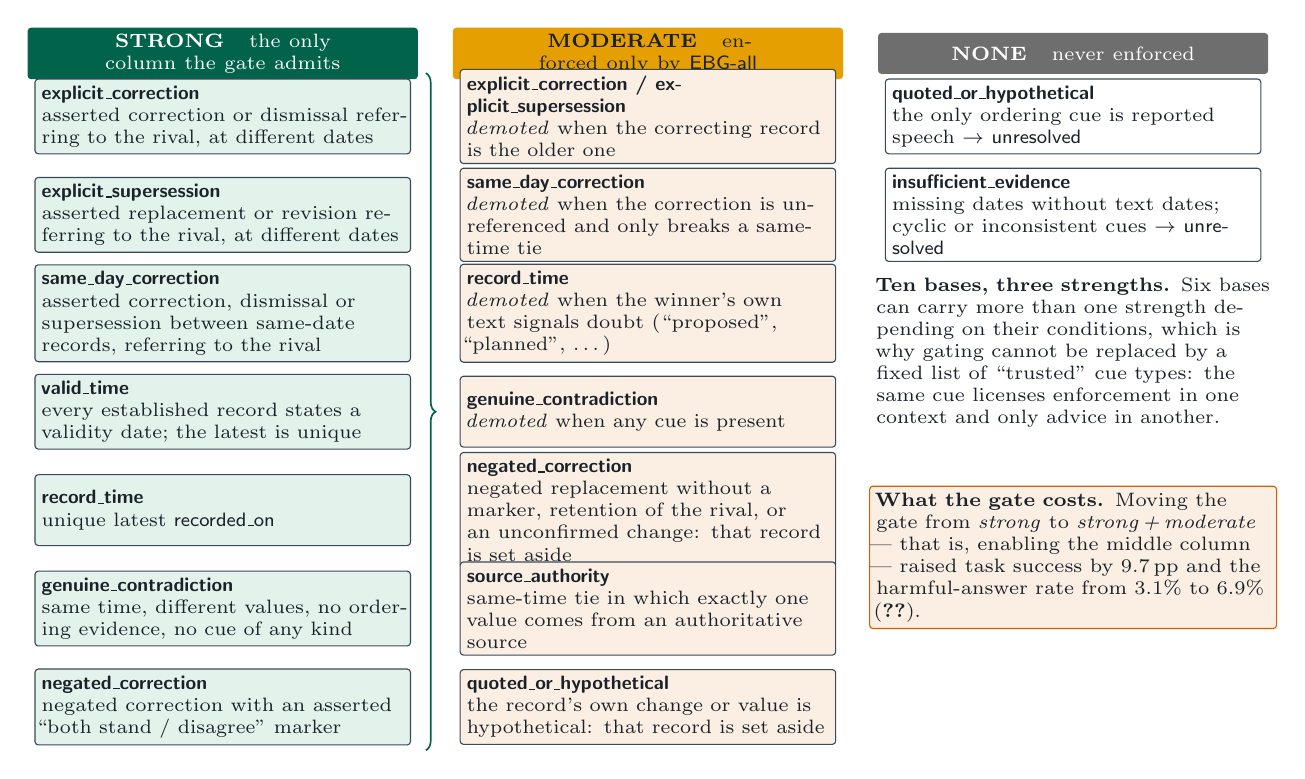
\begin{tikzpicture}[font=\footnotesize, x=1mm, y=1mm,
  base/.style={draw=cBoxEdge, line width=0.4pt, rounded corners=1.2pt, align=left,
               inner sep=2.4pt, text width=46mm, font=\scriptsize, text=cInk, minimum height=9mm},
  hdr/.style={align=center, font=\scriptsize\bfseries, text=white, inner sep=2.2pt,
              rounded corners=1.2pt, minimum height=5.2mm, text width=48mm}]

% ---- column headers: the gate admits the left column only
\node[hdr, fill=cEBG]   (hs) at (26,86) {STRONG\quad\textnormal{\scriptsize the only column the gate admits}};
\node[hdr, fill=cAll, text=cInk] (hm) at (80,86) {MODERATE\quad\textnormal{\scriptsize enforced only by \cond{EBG-all}}};
\node[hdr, fill=cNone]  (hn) at (134,86) {NONE\quad\textnormal{\scriptsize never enforced}};

% ---- strong
\node[base, fill=cAccentFill] (b1) at (26,78)
  {\textbf{\cond{explicit\_correction}}\\asserted correction or dismissal referring to the rival, at different dates};
\node[base, fill=cAccentFill] (b2) at (26,65.5)
  {\textbf{\cond{explicit\_supersession}}\\asserted replacement or revision referring to the rival, at different dates};
\node[base, fill=cAccentFill] (b3) at (26,53)
  {\textbf{\cond{same\_day\_correction}}\\asserted correction, dismissal or supersession between same-date records, referring to the rival};
\node[base, fill=cAccentFill] (b4) at (26,40.5)
  {\textbf{\cond{valid\_time}}\\every established record states a validity date; the latest is unique};
\node[base, fill=cAccentFill] (b5) at (26,28)
  {\textbf{\cond{record\_time}}\\unique latest \cond{recorded\_on}};
\node[base, fill=cAccentFill] (b6) at (26,15.5)
  {\textbf{\cond{genuine\_contradiction}}\\same time, different values, no ordering evidence, no cue of any kind};
\node[base, fill=cAccentFill] (b7) at (26,3)
  {\textbf{\cond{negated\_correction}}\\negated correction with an asserted ``both stand / disagree'' marker};

% ---- moderate (demotions of the same bases, plus two of their own)
\node[base, fill=cWarnFill] (m1) at (80,78)
  {\textbf{\cond{explicit\_correction} / \cond{explicit\_supersession}}\\\emph{demoted} when the correcting record is the older one};
\node[base, fill=cWarnFill] (m2) at (80,65.5)
  {\textbf{\cond{same\_day\_correction}}\\\emph{demoted} when the correction is unreferenced and only breaks a same-time tie};
\node[base, fill=cWarnFill] (m3) at (80,53)
  {\textbf{\cond{record\_time}}\\\emph{demoted} when the winner's own text signals doubt (``proposed'', ``planned'', \ldots)};
\node[base, fill=cWarnFill] (m4) at (80,40.5)
  {\textbf{\cond{genuine\_contradiction}}\\\emph{demoted} when any cue is present};
\node[base, fill=cWarnFill] (m5) at (80,28)
  {\textbf{\cond{negated\_correction}}\\negated replacement without a marker, retention of the rival, or an unconfirmed change: that record is set aside};
\node[base, fill=cWarnFill] (m6) at (80,15.5)
  {\textbf{\cond{source\_authority}}\\same-time tie in which exactly one value comes from an authoritative source};
\node[base, fill=cWarnFill] (m7) at (80,3)
  {\textbf{\cond{quoted\_or\_hypothetical}}\\the record's own change or value is hypothetical: that record is set aside};

% ---- none
\node[base, fill=white] (n1) at (134,78)
  {\textbf{\cond{quoted\_or\_hypothetical}}\\the only ordering cue is reported speech $\rightarrow$ \cond{unresolved}};
\node[base, fill=white] (n2) at (134,65.5)
  {\textbf{\cond{insufficient\_evidence}}\\missing dates without text dates; cyclic or inconsistent cues $\rightarrow$ \cond{unresolved}};

\node[base, draw=none, fill=none, text width=50mm] (note) at (134,48)
  {\textbf{Ten bases, three strengths.} Six bases can carry more than one strength depending on their
   conditions, which is why gating cannot be replaced by a fixed list of ``trusted'' cue types: the same
   cue licenses enforcement in one context and only advice in another.};

\node[base, draw=cEnf, fill=cWarnFill, text width=50mm] (note2) at (134,22)
  {\textbf{What the gate costs.} Moving the gate from \emph{strong} to \emph{strong\,+\,moderate} ---
   that is, enabling the middle column --- raised task success by $9.7$\pp{} and the harmful-answer rate from
   3.1\% to 6.9\% (\Cref{sec:ablations}).};

\draw[decorate, decoration={brace, amplitude=3.5pt}, draw=cEBG, line width=0.6pt]
  (51.8,83.5) -- (51.8,-2.5);
\end{tikzpicture}

\vspace{1mm}
\caption[The ten evidence bases of Evarb-0.2]{%
\textbf{The ten evidence bases, grouped by the strength they can carry.} Names and conditions are verbatim from
the frozen specification; no basis is renamed, added or omitted. The left column is what gated enforcement acts on.
Six of the ten bases appear in more than one column because their strength depends on their conditions --- a
correction whose correcting record is the older one is demoted, an ordering by record date is demoted when the
winning record's own text signals doubt, and a contradiction is demoted when any cue is present. This
context-dependence is the reason the mechanism reports a basis and a strength rather than a verdict.\\
\emph{Accessible description:} a three-column layout headed STRONG, MODERATE and NONE, holding seven, seven and two
entries respectively; a brace marks the left column as the only one the gate admits.\\
\emph{Source:} \srcfile{EVIDENCE_ARBITRATION_SPEC.md} \S3; \srcfile{evarb/arbiter.py}.}
\label{fig:bases}
\end{figure}


\paragraph{What the agent sees.} Labels are attached to each retrieved record in the \cond{memory\_search} result:
a status, the evidence basis in words, a certainty (\cond{established}, \cond{likely}, \cond{not established},
mapped from strength) and, where relevant, \cond{superseded\_by}, \cond{conflicts\_with}, \cond{valid\_from} and a
note. A superseded record is shown as \cond{historical} when the question asks about an earlier time, because
whether a record is historical depends on the question rather than on the records. An order the evidence cannot
establish is shown as \cond{unresolved}, with the instruction to read the record texts --- never as
``conflicting'', because in the pilot small models followed wrong cautionary labels.

\subsection{The basis-gated policy}

The policy is evaluated when the agent submits, and applies only to \emph{anchored} groups: groups the agent
retrieved whose entity is named in the question. It never sees the gold answer, and model identity is not an input.
The first matching rule wins:

\begin{description}[leftmargin=2.2em,itemsep=1pt,topsep=2pt,font=\normalfont\sffamily]
\item[P3] no \cond{memory\_search} and no successful registry result $\rightarrow$ request evidence (search memory;
if nothing relevant, the previous submission stands);
\item[P1] current question, and the answer equals a superseded value and not the current one $\rightarrow$ enforce
if enforceable, else advise;
\item[P2] current question, status \cond{conflict}, and every anchored multi-value group is resolved $\rightarrow$
enforce if all are enforceable, else advise;
\item[P4] the answer equals a value of a contradictory group and there is no registry result $\rightarrow$ enforce
toward \cond{conflict} if enforceable, else advise;
\item[--] anything else, including every unresolved group $\rightarrow$ no action.
\end{description}

\paragraph{Gating} is the single switch this paper is about. A resolution is \emph{enforceable} in mode
\cond{gated} if its strength is strong; in mode \cond{all} if it is strong \emph{or} moderate; in mode \cond{none},
never. \cond{EBG} uses \cond{gated}; \cond{EBG-all} uses \cond{all}; the advisory conditions use \cond{none}.

\paragraph{Notices.} A run receives at most one notice. It names the records involved and states the evidence basis
truthfully --- a same-date correction is described as a correction, not as an ordering by date. The agent may
resubmit; the policy never changes an answer itself.

\paragraph{Safe submission.} If the submission after a notice is unparsable or missing, or the step budget runs
out, the final answer reverts to the pre-notice submission. This bounds the cost of a notice: it can turn one
parsable answer into another, but it cannot turn a parsable answer into a format or step-limit failure.

\subsection{Conditions}
\label{sec:conditions}

\begin{table}[t]
\centering
\caption{The twelve conditions. All twelve run in every cell. \cond{EBG} is the proposed condition; \cond{RT} is
the pre-registered primary comparator. ``Enforced'' means the policy may block or correct a submission that
disagrees with the arbitration; ``gated'' restricts that to resolutions of strong strength.}
\label{tab:conditions}
\footnotesize
\setlength{\tabcolsep}{3pt}
\begin{tabular}{@{}llllccl@{}}
\toprule
\textbf{Condition} & \textbf{Labels shown} & \textbf{Enforcement} & \textbf{Search} & \textbf{Safe} & \textbf{Role} \\
 & & & \textbf{first} & \textbf{submit} & \\
\midrule
\cond{B}   & none (memory only)      & ---                     & ---  & ---  & no-label baseline \\
\cond{G}   & metadata (record date)  & ---                     & ---  & ---  & advisory metadata \\
\cond{R}   & metadata                & every label             & yes  & no   & prior enforcement \\
\cond{T}   & temporal arbiter        & ---                     & ---  & ---  & advisory temporal labels \\
\cond{RT}  & temporal arbiter        & every label             & yes  & no   & \textbf{primary comparator} \\
\midrule
\cond{EB}  & evidence basis          & ---                     & ---  & ---  & labels only, advisory \\
\textbf{\cond{EBG}} & \textbf{evidence basis} & \textbf{gated (strong only)} & \textbf{yes} & \textbf{yes} & \textbf{proposed} \\
\cond{EBG-all}      & evidence basis  & strong \emph{and} moderate & yes & yes & ablation: the gate \\
\cond{EBG-unsafe}   & evidence basis  & gated                   & yes  & no   & ablation: safe submission \\
\cond{EBG-noR3}     & evidence basis  & gated                   & no   & yes  & ablation: search-before-submit \\
\midrule
\cond{LA}  & LLM arbiter             & ---                     & ---  & ---  & LLM arbiter, advisory \\
\cond{LG}  & LLM arbiter             & gated                   & yes  & yes  & LLM arbiter, EBG policy \\
\bottomrule
\end{tabular}
\end{table}


All twelve conditions run in every cell. They are constructed so that each comparison of interest differs in one
design element where possible: \cond{EBG} vs \cond{EB} isolates enforcement, \cond{EBG} vs \cond{EBG-all} isolates
gating, \cond{EBG} vs \cond{EBG-unsafe} isolates safe submission, \cond{EBG} vs \cond{EBG-noR3} isolates
search-before-submit, and \cond{EBG} vs \cond{LG} isolates \emph{who} arbitrates while holding the policy fixed.

The pre-registered primary contrast, \cond{EBG} $-$ \cond{RT}, is deliberately not of that kind: it compares the
proposed condition with the strongest prior enforcing condition and therefore changes the arbiter, the gating, the
notice wording and safe submission together. It cannot attribute an effect to any one of them. The ablations in
\Cref{sec:ablations} do the attribution, and they are exploratory.

\paragraph{Baselines.} \cond{G} and \cond{R} use metadata-only labels that order records by \cond{recorded\_on}
alone and label same-date disagreements as conflicting. \cond{T} and \cond{RT} use the earlier temporal arbiter:
it orders by text validity dates where every competing record has one, else by a unique latest \cond{recorded\_on},
breaking ties by a correction cue naming the rival's value, and otherwise reports no ordering evidence. It has no
negation, quotation or modality scope, and its labels carry no strength --- which is exactly what gating needs and
cannot get from it. \cond{R} and \cond{RT} enforce every label they produce and have no safe submission.
\cond{LA} and \cond{LG} use the agent's own model as arbiter, filling the same output schema from a prompt that
states the same evidence rules in plain language; unparsable or inconsistent output becomes \cond{unresolved} and
is counted as a format failure.

\section{Experimental design and pre-registration}
\label{sec:design}

% Figure 4 -- experimental design: the sealed benchmark, the 18-cell run matrix, and the analysis arms.
% Counts from PHASE3/PHASE3_DECISIONS.json, PHASE3/ANALYSIS/COMPLETENESS.json and PHASE2/FREEZE_eval3.json.
\begin{figure}[t]
\centering
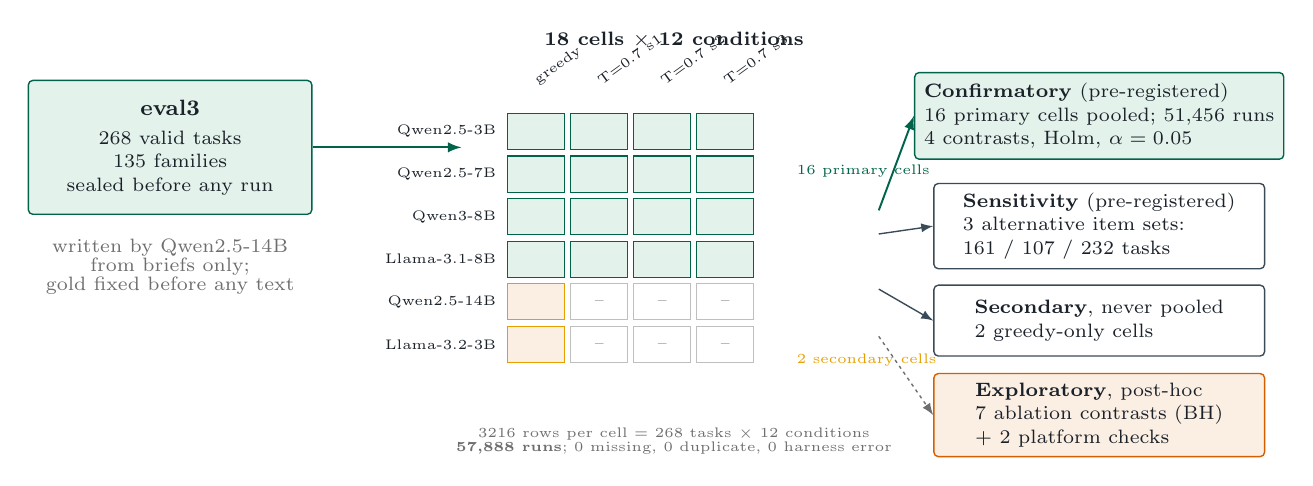
\begin{tikzpicture}[font=\footnotesize, x=1mm, y=1mm,
  gcellp/.style={draw=cEBG, fill=cAccentFill, line width=0.4pt, minimum width=7.2mm, minimum height=4.6mm,
                inner sep=0pt, font=\tiny, text=cInk},
  gcells/.style={gcellp, draw=cAll, fill=cWarnFill},
  gcellx/.style={draw=cNeutral, fill=white, line width=0.3pt, minimum width=7.2mm, minimum height=4.6mm,
                inner sep=0pt, font=\tiny, text=cNone}]

% ---------------- benchmark
\node[blkacc, minimum width=36mm, minimum height=17mm, align=center] (bench) at (20,48)
  {\textbf{eval3}\\[1pt]\scriptsize 268 valid tasks\\[-1pt]\scriptsize 135 families\\[-1pt]\scriptsize sealed before any run};
\node[lbl, text=cNone, align=center, anchor=north] at (20,37)
  {\scriptsize written by Qwen2.5-14B\\[-1pt]\scriptsize from briefs only;\\[-1pt]\scriptsize gold fixed before any text};

% ---------------- the 18-cell matrix
\node[lbl, anchor=south, font=\scriptsize\bfseries] at (84,60) {18 cells $\times$ 12 conditions};
\foreach \d [count=\i from 0] in {greedy, {T=0.7 s1}, {T=0.7 s2}, {T=0.7 s3}}
  \node[lbl, rotate=36, anchor=west, font=\tiny] at (66+\i*8,56) {\d};
\foreach \m [count=\j from 0] in {{Qwen2.5-3B}, {Qwen2.5-7B}, {Qwen3-8B}, {Llama-3.1-8B}, {Qwen2.5-14B}, {Llama-3.2-3B}}
  \node[lbl, anchor=east, font=\tiny] at (62,50-\j*5.4) {\m};
\foreach \j in {0,1,2,3}
  \foreach \i in {0,1,2,3}
    \node[gcellp] at (66.5+\i*8,50-\j*5.4) {};
\node[gcells] at (66.5,50-4*5.4) {};
\node[gcells] at (66.5,50-5*5.4) {};
\foreach \j in {4,5}
  \foreach \i in {1,2,3}
    \node[gcellx] at (66.5+\i*8,50-\j*5.4) {--};
\node[lbl, text=cEBG, anchor=west, font=\tiny] at (99,45) {16 primary cells};
\node[lbl, text=cAll, anchor=west, font=\tiny] at (99,21) {2 secondary cells};
\node[lbl, anchor=north, align=center, font=\tiny, text=cNone] at (84,13)
  {3216 rows per cell $=$ 268 tasks $\times$ 12 conditions\\[-1pt]\textbf{57{,}888 runs}; 0 missing, 0 duplicate, 0 harness error};

% ---------------- analysis arms
\node[blkacc, minimum width=42mm, minimum height=11mm, align=left] (prim) at (138,52)
  {\scriptsize\textbf{Confirmatory} (pre-registered)\\[-1pt]\scriptsize 16 primary cells pooled; 51{,}456 runs\\[-1pt]\scriptsize 4 contrasts, Holm, $\alpha=0.05$};
\node[blkplain, minimum width=42mm, minimum height=10mm, align=left] (sens) at (138,38)
  {\scriptsize\textbf{Sensitivity} (pre-registered)\\[-1pt]\scriptsize 3 alternative item sets:\\[-1pt]\scriptsize 161 / 107 / 232 tasks};
\node[blkplain, minimum width=42mm, minimum height=9mm, align=left] (sec) at (138,26)
  {\scriptsize\textbf{Secondary}, never pooled\\[-1pt]\scriptsize 2 greedy-only cells};
\node[blkwarn, minimum width=42mm, minimum height=10mm, align=left] (expl) at (138,14)
  {\scriptsize\textbf{Exploratory}, post-hoc\\[-1pt]\scriptsize 7 ablation contrasts (BH)\\[-1pt]\scriptsize $+$ 2 platform checks};

\draw[flowacc] (bench.east) -- (57,48);
\draw[flowacc] (110,40) -- (prim.west);
\draw[flow] (110,37) -- (sens.west);
\draw[flow] (110,30) -- (sec.west);
\draw[flowback] (110,24) -- (expl.west);
\end{tikzpicture}

\vspace{1mm}
\caption[Experimental design]{%
\textbf{Experimental design.} A sealed benchmark, a fully crossed run matrix, and four analysis arms that are kept
separate throughout the paper. Every one of the six models ran all twelve conditions on all 268 tasks; the four
primary models ran greedy decoding and three $T=0.7$ seeds, and the two secondary models ran greedy only and are
never pooled with the primary ones. The matrix completed with no missing pair, no duplicate and no harness error,
so the pre-registered missing-run rule never had to be applied. Only the first arm supports a confirmatory claim:
the sensitivity analyses were pre-registered but are reported as sensitivity, and everything in the fourth arm is
exploratory, with the two platform checks additionally post-hoc (\Cref{sec:statistics}).\\
\emph{Accessible description:} three panels left to right --- the sealed benchmark, a six-by-four grid of cells in
which the top four rows are full and the bottom two have only their first column filled, and a stack of four
analysis arms.\\
\emph{Source:} \srcfile{PHASE3/ANALYSIS/COMPLETENESS.json}; \srcfile{PHASE2/FREEZE_eval3.json};
\srcfile{PHASE3/PHASE3_DECISIONS.json}.}
\label{fig:design}
\end{figure}


\subsection{What was frozen, and when}

The mechanism was frozen on 14 November 2026: nine arbiter modules, the runner, the analysis script and the
component evaluator, with three frozen dependencies, recorded as a hash manifest. The evaluation set was sealed on
16 November, its gold fixed before any agent saw it. The analysis was pre-registered and frozen on 17 November,
with its own SHA-256 recorded in the seal manifest, \emph{before} the first confirmatory run. Every job then
refused to start unless the mechanism files matched the freeze, the sealed directory passed its checksum, and the
pre-registration hash matched the recorded value; all 20 job starts of the campaign passed all three.

\subsection{Hypotheses}

The pre-registration fixes four success contrasts and one harm test, in this order, with Holm correction over the
four:

\begin{description}[leftmargin=4.4em,itemsep=1pt,topsep=2pt,font=\normalfont\sffamily]
\item[H-primary] \cond{EBG} yields higher task success than \cond{RT} (enforced record-and-temporal labels).
\item[S1] \cond{EBG} yields higher task success than \cond{T} (advisory temporal labels).
\item[S2] \cond{EBG} yields higher task success than \cond{LG} (LLM arbiter under the same gated policy).
\item[S3] \cond{EBG} yields higher task success than \cond{B} (memory without labels).
\item[S4] \cond{EBG}'s harmful-answer rate is \emph{no higher} than \cond{RT}'s.
\end{description}

S4 is a test the mechanism can fail, not one it can pass: its possible verdicts are ``falsified'' and ``not
falsified''. The pre-registration also named three outcomes that would falsify the contribution ---
\cond{EBG} $-$ \cond{RT} $\le 0$, \cond{EBG} $-$ \cond{LG} $\le 0$, and \cond{EBG}'s harmful rate exceeding
\cond{RT}'s --- and required all of them to be reported whatever their sign.

\subsection{Unit, clustering and test}

The unit of analysis is the task. Success per task is the mean over a model's decodings; contrasts are paired
within model and decoding. Families --- (category, attribute) pairs, 135 of them among the valid items --- are the
clustering unit, because tasks within a family share a template and are not independent. The test is a two-sided
sign-flip permutation of family-level summed differences with families pooled across models, so a family's sign is
flipped for all models together; with 135 families exact enumeration is infeasible and the analysis uses 100{,}000
seeded Monte-Carlo draws, whose smallest attainable estimate is $1\times10^{-5}$
\citep{good2005permutation}. Confidence intervals are 95\% percentile bootstraps over families with 10{,}000
seeded resamples \citep{efron1979bootstrap,field2007clustered}. Holm's step-down procedure controls the familywise
error rate over the four pre-registered contrasts at $\alpha=0.05$ \citep{holm1979simple}; every other contrast is
exploratory and reported with Benjamini--Hochberg adjustment \citep{benjamini1995fdr}.

\subsection{Exclusions and missing runs}

There are \textbf{no run-level exclusions}. Unparsable outputs, harness errors and step-limit hits are failures. A
(task, condition) pair with no row, or with a harness error, is scored as a failure and counted separately; a cell
with more than 5\% missing pairs is re-submitted once, with the runner resuming. In this campaign no pair was
missing and no harness error occurred, so these rules never had to be applied.

\subsection{A documented inconsistency in the frozen document}

The pre-registration is internally inconsistent about the primary item set. Its \S5 states that the primary set is
every mechanically valid item; its \S6 and \S8 still contain an earlier rule under which flagged items --- those
with annotator disagreement or low confidence --- would be excluded from the primary analysis. The \S6 and \S8
wording was not updated when \S5 was revised.

We follow \S5 and the recorded primary-set decision: the primary set is all 268 valid items, and the
double-agreement and flagged subsets are reported as sensitivity analyses. We report this as a defect in the frozen
document rather than correct it silently, and \Cref{tab:sensitivity} gives the numbers a reader who prefers the
\S6 reading would need: the four contrasts are $+14.3$, $+12.7$, $+19.7$ and $+14.7$\pp{} on the 161-task
double-agreement subset, all with intervals above zero and Holm-adjusted $p<0.05$. The conclusions do not depend
on which reading is taken.

\section{Dataset and benchmark construction}
\label{sec:dataset}

\subsection{How eval3 was built}

The evaluation set, \textbf{eval3}, was constructed so that its gold answers are fixed \emph{before any text
exists}. A skeleton generator produces groups of records about one (entity, attribute) pair --- the structure, the
record dates, the intended relation between the records and therefore the correct answer --- as structured briefs
with no prose. Only then were the record texts written, by Qwen2.5-14B-Instruct from the briefs alone. The writer
input contained no gold field, no date or source field and no label words, and the writer was required to keep each
record's own value verbatim and to write date \emph{values} in ISO form so that the mechanical validator would not
reject correct long-form dates. Questions about the current state use templates shared with every split.

A mechanical validator then rejected items whose text failed to carry its own value, whose value appeared in the
question, or that contained no entity. Of 276 skeleton items, \textbf{268 remained valid}, spanning
\textbf{135 families}. The eight exclusions are recorded by identifier.

The set was sealed on the cluster before any confirmatory run: a hash manifest over the task file, the skeleton,
the groups and the annotations, with the manifest's own hash recorded in the freeze record. The runner refuses any
task file whose hash differs from the sealed one.

\subsection{Annotation, and why it is a sensitivity analysis rather than a filter}

eval3 has \textbf{no human validation}. It was annotated blind by two model annotators against the three gold
classes. Agreement with gold was 174 of 268 ($\kappa=0.471$) for one annotator and 232 of 268 ($\kappa=0.767$) for
the other \citep{cohen1960kappa}; 161 items have double agreement and 107 are flagged by at least one annotator.

These numbers are annotation statistics, not outcomes, and they are reported here because they bound what the set
can support. We do \emph{not} filter on them: the primary analysis uses all 268 valid items, and the
double-agreement subset (161), the flagged complement (107) and the subset agreed by the stronger annotator (232)
are three separate sensitivity analyses (\Cref{tab:sensitivity}). Effects are somewhat \emph{larger} on the
flagged complement ($+21.3$\pp{} on H-primary) than on the double-agreement subset ($+14.3$\pp), which is the
opposite of what an ``annotator noise inflates the effect'' account would predict.

\subsection{What the set is, and is not}

eval3 is synthetic, templated, English-only, ISO-dated, model-written and model-annotated. It was built to be
sealed and pre-registered against, and that is the only claim we make for it. It is not a benchmark of record: the
closest external set, STALE, has 400 expert-validated scenarios, and DISCERN's evaluation set is human-vetted
\citep{chao2026stale,ahuja2026discern}. One consequence is worth stating plainly: the writer, Qwen2.5-14B, is also
one of the annotators and one of the evaluated secondary models, so that model's results carry a dependence the
others do not. We report it separately and never pool it.

A second consequence runs the other way. Because eval3 \emph{includes} explicitly signalled invalidation --- the
corrections, supersessions and negations a lexical arbiter is built to read --- it is favourable ground for Evarb
by construction. STALE deliberately excludes those cases, which makes it the natural external test of what this
mechanism cannot do, and an obvious next step rather than a result we can claim here.

\section{Experimental setup and baselines}
\label{sec:setup}

\begin{table}[t]
\centering
\caption{Models, decodings and the resulting run matrix. All six models ran all twelve conditions on all 268
tasks. Snapshot hashes, framework versions and the hashes of all 14 mechanism files are recorded in every run
manifest and released with the artifact package.}
\label{tab:setup}
\footnotesize
\setlength{\tabcolsep}{5pt}
\begin{tabular}{@{}llccr@{}}
\toprule
\textbf{Model} & \textbf{Role} & \textbf{Decodings} & \textbf{Cells} & \textbf{Runs} \\
\midrule
Qwen2.5-3B \citep{qwen2024qwen25}      & primary & greedy $+$ 3 seeds & 4 & 12\,864 \\
Qwen2.5-7B \citep{qwen2024qwen25}      & primary & greedy $+$ 3 seeds & 4 & 12\,864 \\
Qwen3-8B \citep{yang2025qwen3}                  & primary & greedy $+$ 3 seeds & 4 & 12\,864 \\
Llama-3.1-8B \citep{grattafiori2024llama3} & primary & greedy $+$ 3 seeds & 4 & 12\,864 \\
\midrule
Qwen2.5-14B \citep{qwen2024qwen25}     & secondary & greedy & 1 & 3\,216 \\
Llama-3.2-3B \citep{grattafiori2024llama3} & format-limited & greedy & 1 & 3\,216 \\
\midrule
\multicolumn{3}{@{}l}{\textbf{Total}} & \textbf{18} & \textbf{57\,888} \\
\bottomrule
\end{tabular}

\vspace{2pt}
{\footnotesize bfloat16 on one 48\,GB GPU; at most 700 new tokens per call; greedy decoding uses base seed
20261111, sampled decoding uses $T=0.7$, top-$p=0.9$. Llama-3.2-3B failed the pre-registered readiness criterion
before the campaign and is reported separately throughout. Source:
\srcfile{PHASE3/results/execution.csv}.}
\end{table}


\subsection{Models and decoding}

Six open-weight instruction-tuned models were run, four as primary and two as secondary
(\Cref{tab:setup}). Models run locally in bfloat16 on a single 48\,GB GPU, loaded from pinned snapshots, with at
most 700 new tokens per call and chat templates with thinking disabled where supported. Greedy conditions use base
seed 20261111; sampled conditions use $T=0.7$ with top-$p=0.9$ and seeds 1, 2 and 3. Tool calls are parsed from
the raw generation by the project's own parser, and the raw text, parser version and parse path are logged, so a
parse failure is visible as such rather than silently scored as a wrong answer.

Llama-3.2-3B failed the pre-registered readiness criterion before the campaign --- it does not reliably produce the
tool-call format --- and was retained as a format-limited secondary cell, reported separately and never pooled.
That decision was made and recorded before any confirmatory run.

\subsection{Baselines}

The comparison set is built from the mechanisms this work is meant to improve on, not from weak straw men.

\begin{description}[leftmargin=3.2em,itemsep=1.5pt,topsep=2pt,font=\normalfont\sffamily]
\item[\cond{B}] Memory with no labels: the agent reads the retrieved records and decides. This is the floor that
any labelling must beat.
\item[\cond{G}, \cond{R}] Metadata labels that order records by record date alone and mark same-date
disagreements as conflicting, advisory (\cond{G}) and enforced (\cond{R}). This is the design that motivated the
study.
\item[\cond{T}, \cond{RT}] A lexical temporal arbiter that orders by stated validity dates where all competing
records have them, else by a unique latest record date, breaking ties on a correction cue naming the rival's
value. It has no negation, quotation or modality scope and its labels carry no strength --- which is exactly what
gating would need and cannot get from it. \cond{RT} enforces every label it produces and has no safe submission;
it is the pre-registered primary comparator.
\item[\cond{LA}, \cond{LG}] The agent's own model as arbiter, filling the same output schema from a prompt
stating the same evidence rules in plain language, advisory (\cond{LA}) and under the identical gated policy
(\cond{LG}). Unparsable or inconsistent arbiter output becomes \cond{unresolved} and is counted as a format
failure. Arbiter calls are logged and counted separately from the agent's.
\end{description}

\subsection{Scoring}

A frozen scorer classifies each run. Task success requires the submitted answer to match the gold answer, where the
gold may be a value, the literal \cond{conflict}, or an abstention. Four outcomes count as \textbf{harmful}:
\cond{wrong\_value}, \cond{stale\_value}, \cond{unsupported\_claim} and \cond{arbitrary\_pick}. The descriptive
measures also report conflict preservation (the share of genuinely unresolvable groups still reported as a
conflict), false resolution (the share for which a value is asserted instead), unnecessary abstention, format
failure, step-limit exhaustion, and per-run tool, model and arbiter call counts with latency.

\subsection{Execution}

Each cell ran as a single scheduled job on one GPU, with a controller keeping at most two cells in flight and
resubmitting any cell that stopped short. A separate CPU-only job then ran the integrity gates, the staging, the
verification, the frozen analysis, the independent cross-check, the report generation and a final hash manifest,
stopping at the first failure. No interactive session takes part in any of this, which is what makes the chain in
\Cref{fig:integrity} auditable after the fact.

\section{Results}
\label{sec:results}

Every number in this section comes from the frozen analysis run over the 18 completed cells. All 18 hold exactly
$268\times12=3216$ rows --- 57{,}888 in total --- with no missing pair, no duplicate, no unparsable line and no
harness error. The confirmatory analysis pools the four primary models over four decodings: 268 tasks, 135
families, 51{,}456 scored runs. An independent re-implementation recomputed the 60 model $\times$ condition success
counts and the four primary effect sizes by a different route and agrees with the frozen analysis exactly.

\begin{table}[t]
\centering
\caption{The pre-registered confirmatory results. Differences are in percentage points of task success, paired
within model and decoding, pooled over the four primary models (268 tasks, 135 families, 51{,}456 runs).
Intervals are 95\% percentile bootstraps over families (10{,}000 seeded resamples); $p$ is a two-sided sign-flip
permutation test on family-level summed differences (100{,}000 seeded draws, Monte-Carlo floor
$1\times10^{-5}$); Holm correction is over these four contrasts at $\alpha=0.05$. S4 is a harm test and is
reported as \emph{not falsified}, not as a fifth supported hypothesis.}
\label{tab:primary}
\small
\setlength{\tabcolsep}{5pt}
\begin{tabular}{@{}llrcrrl@{}}
\toprule
& \textbf{Contrast} & \textbf{Diff.\ (pp)} & \textbf{95\% CI} & $\boldsymbol p$ & $\boldsymbol{p_{\text{Holm}}}$ & \textbf{Verdict} \\
\midrule
\textbf{H-primary} & \cond{EBG} $-$ \cond{RT} & $+17.1$ & \ci{12.2}{22.1} & $1\!\times\!10^{-5}$ & $4\!\times\!10^{-5}$ & \textbf{supported} \\
S1 & \cond{EBG} $-$ \cond{T}  & $+14.5$ & \ci{10.5}{18.6} & $1\!\times\!10^{-5}$ & $4\!\times\!10^{-5}$ & supported \\
S2 & \cond{EBG} $-$ \cond{LG} & $+15.9$ & \ci{10.4}{21.2} & $1\!\times\!10^{-5}$ & $4\!\times\!10^{-5}$ & supported \\
S3 & \cond{EBG} $-$ \cond{B}  & $+15.3$ & \ci{10.3}{20.5} & $1\!\times\!10^{-5}$ & $4\!\times\!10^{-5}$ & supported \\
\midrule
S4 & \cond{EBG} $-$ \cond{RT}, harmful & $-19.4$ & \ci{-24.6}{-14.6} & $1\!\times\!10^{-5}$ & --- & not falsified \\
\bottomrule
\end{tabular}

\vspace{2pt}
{\footnotesize Harmful answers: \cond{EBG} 135/4288 (3.1\%) against \cond{RT} 968/4288 (22.6\%). Arbitrary picks:
13 against 252. All four success contrasts reach the Monte-Carlo floor before correction, so the Holm-adjusted
values are $4\times10^{-5}$ for all four. Source: \srcfile{PHASE3/PHASE3_DECISIONS.json}.}
\end{table}

% Figure 5 -- forest plot of the four pre-registered contrasts.
% Data: figures/data/fig5_forest_primary.dat and fig5c_double_agreement.dat
% Generated by PHASE5_PUBLICATION/figures_source/make_figure_data.py from
% PHASE3/PHASE3_DECISIONS.json and PHASE3/ANALYSIS/{CONFIRMATORY_primary_cells,SENSITIVITY_*}.json
\begin{figure}[t]
\centering
\begin{tikzpicture}
\begin{axis}[
  paperaxis,
  width=0.70\linewidth, height=4.6cm,
  xlabel={Difference in task success (percentage points), EBG $-$ comparator},
  xmin=-1.5, xmax=41,
  ymin=0.45, ymax=4.75,
  ytick={4,3,2,1},
  yticklabels={%
    {\textbf{H-primary}: \cond{EBG}$-$\cond{RT}},
    {S1: \cond{EBG}$-$\cond{T}},
    {S2: \cond{EBG}$-$\cond{LG}},
    {S3: \cond{EBG}$-$\cond{B}}},
  yticklabel style={font=\scriptsize, align=right},
  xmajorgrids, xtick={0,5,10,15,20,25},
  clip=false,
]
\addplot[draw=cInk, line width=0.6pt, dashed] coordinates {(0,0.45) (0,4.55)};
\node[lbl, text=cInk, anchor=south] at (axis cs:0,4.56) {\scriptsize no effect};

% pre-registered sensitivity item set (161-task double-agreement subset), offset upward
\addplot[only marks, mark=o, mark size=1.3pt, draw=cNone, line width=0.5pt,
         error bars/.cd, x dir=both, x explicit,
         error bar style={draw=cNone, line width=0.4pt}]
  table[col sep=tab, x=diff, y expr={\thisrow{y}+0.23},
        x error plus expr={\thisrow{hi}-\thisrow{diff}},
        x error minus expr={\thisrow{diff}-\thisrow{lo}}]
  {figures/data/fig5c_double_agreement.dat};

\addplot[only marks, mark=*, mark size=2.0pt, draw=cEBG, fill=cEBG,
         error bars/.cd, x dir=both, x explicit, error bar style={draw=cEBG, line width=0.9pt},
         error mark options={draw=cEBG, line width=0.9pt, mark size=1.8pt}]
  table[col sep=tab, x=diff, y=y,
        x error plus expr={\thisrow{hi}-\thisrow{diff}},
        x error minus expr={\thisrow{diff}-\thisrow{lo}}]
  {figures/data/fig5_forest_primary.dat};

\node[lbl, anchor=west, text=cEBG] at (axis cs:26.5,4) {$+17.1$\ \ci{12.2}{22.1}};
\node[lbl, anchor=west, text=cEBG] at (axis cs:26.5,3) {$+14.5$\ \ci{10.5}{18.6}};
\node[lbl, anchor=west, text=cEBG] at (axis cs:26.5,2) {$+15.9$\ \ci{10.4}{21.2}};
\node[lbl, anchor=west, text=cEBG] at (axis cs:26.5,1) {$+15.3$\ \ci{10.3}{20.5}};
\node[lbl, anchor=west, text=cNone] at (axis cs:26.5,4.45) {\scriptsize confirmatory estimate};
\end{axis}
\end{tikzpicture}

\vspace{-1mm}
\caption[Pre-registered confirmatory contrasts]{%
\textbf{The four pre-registered contrasts.} Difference in task success between evidence-basis gated enforcement
(\cond{EBG}) and each comparator, in percentage points; positive values favour \cond{EBG}. Filled markers are the
confirmatory estimates on the primary item set (268 tasks, 135 families, 51{,}456 runs); bars are 95\% percentile
bootstrap intervals over families (10{,}000 seeded resamples). All four intervals exclude zero and all four
Holm-adjusted $p$-values are $4\times10^{-5}$ (two-sided sign-flip permutation on family-level summed differences,
100{,}000 seeded draws; the Monte-Carlo floor is $1\times10^{-5}$). Open grey markers above each estimate show the
same contrast on the 161-task double-agreement subset, a pre-registered sensitivity analysis. Comparators:
\cond{RT} enforced record-conflict and temporal labels, \cond{T} advisory temporal labels, \cond{LG} an LLM arbiter
under the same gated policy, \cond{B} memory with no labels.\\
\emph{Accessible description:} a four-row forest plot; every estimate and its whole interval lie to the right of
the zero line, between about $+10$ and $+22$ percentage points.\\
\emph{Source:} \srcfile{PHASE3/PHASE3_DECISIONS.json}; plotted from
\srcfile{figures/data/fig5_forest_primary.dat}.}
\label{fig:forest}
\end{figure}


\subsection{The four pre-registered contrasts}

All four are supported (\Cref{tab:primary}, \Cref{fig:forest}). Gated evidence-basis arbitration raised task
success over enforced record-and-temporal labels by $17.1$\pp{} \ci{12.2}{22.1}, over advisory temporal labels by
$14.5$\pp{} \ci{10.5}{18.6}, over an LLM arbiter under the same gated policy by $15.9$\pp{} \ci{10.4}{21.2}, and
over unlabelled memory by $15.3$\pp{} \ci{10.3}{20.5}. All four reach the Monte-Carlo floor before correction, so
Holm leaves them at $4\times10^{-5}$. Family support is lopsided rather than marginal: for \cond{EBG} $-$
\cond{RT}, between 41 and 66 families per model favour \cond{EBG} against between 3 and 25 against.

\subsection{Harm}

S4 asked whether \cond{EBG}'s harmful-answer rate is no higher than \cond{RT}'s. It is substantially lower:
\textbf{3.1\%} of \cond{EBG} runs were harmful (135 of 4288) against \textbf{22.6\%} for \cond{RT} (968 of 4288),
a paired difference of $-19.4$\pp{} \ci{-24.6}{-14.6}. Arbitrary picks --- the specific harm that motivated the
mechanism --- fall from 252 runs to 13. The pre-registered verdict is \textbf{not falsified}: the interval for the
harm difference does not lie above zero and \cond{EBG}'s arbitrary picks do not exceed \cond{RT}'s. None of the
three pre-registered falsification criteria was met.

% Figure 6 -- the accuracy / harm trade-off. Both panels use zero-based axes.
% Data: figures/data/fig6_accuracy_harm.dat, fig6b_conflict_handling.dat
% Generated by PHASE5_PUBLICATION/figures_source/make_figure_data.py from
% PHASE3/results/per_model_config.csv (primary models) and PHASE3/ANALYSIS/METRICS.json
\begin{figure}[t]
\centering
\begin{tikzpicture}
% ---------------- panel (a): success and harm side by side, both measured from zero
\begin{axis}[
  paperaxis, name=panelA,
  width=0.40\linewidth, height=7.0cm,
  xbar=0pt, bar width=2.4pt,
  xmin=0, xmax=78,
  xlabel={\% of runs},
  symbolic y coords={EBG-noR3,EBG-unsafe,EBG-all,EBG,EB,LG,LA,RT,R,T,G,B},
  ytick=data,
  y tick label style={font=\scriptsize},
  xmajorgrids, xtick={0,20,40,60},
  enlarge y limits=0.05,
  legend style={at={(0.5,-0.19)}, anchor=north, legend columns=2, draw=cNeutral},
  legend cell align=left,
  title={(a) success and harm, from zero},
]
\addplot[draw=cAcc, fill=cAcc, fill opacity=0.85]
  table[col sep=tab, x=success, y=config] {figures/data/fig6_accuracy_harm.dat};
\addplot[draw=cHarm, fill=cHarm, fill opacity=0.85, postaction={pattern=north east lines, pattern color=white}]
  table[col sep=tab, x=harmful, y=config] {figures/data/fig6_accuracy_harm.dat};
\legend{task success, harmful answer}
\end{axis}

% ---------------- panel (b): the trade-off plane
\begin{axis}[
  paperaxis, name=panelB, at={(panelA.right of east)}, anchor=left of west, xshift=8mm,
  width=0.47\linewidth, height=7.0cm,
  xlabel={task success (\% of runs) $\rightarrow$ better},
  ylabel={harmful answers (\% of runs) $\rightarrow$ worse},
  xmin=0, xmax=82, ymin=0, ymax=26,
  xtick={0,20,40,60,80}, ytick={0,5,10,15,20,25},
  xmajorgrids, ymajorgrids,
  title={(b) the twelve conditions in the trade-off plane},
  clip=false,
]
% the trade we draw attention to: gating gives up accuracy to buy safety
\draw[->, >=latex, line width=1.1pt, draw=cAll] (axis cs:61.3,3.1) -- (axis cs:71.1,6.9);
\draw[draw=cAll, line width=0.4pt] (axis cs:67,5.1) -- (axis cs:62,13.5);
\node[lbl, text=cAll, anchor=south, align=center] at (axis cs:62,13.8)
  {\scriptsize \textbf{drop the gate}\\[-1pt]\scriptsize $+9.7$\pp{} success\\[-1pt]\scriptsize $+3.8$\pp{} harm};

\addplot[only marks, mark=*, mark size=2.0pt, draw=cNone, fill=cNone] coordinates {(46.0,7.0)};
\node[lbl, anchor=north east] at (axis cs:46.0,7.0) {B\,};
\addplot[only marks, mark=square*, mark size=1.9pt, draw=cAdv!65!black, fill=cAdv]
  coordinates {(43.5,7.9) (46.9,7.4)};
\node[lbl, anchor=south east] at (axis cs:43.5,7.9) {G\,};
\node[lbl, anchor=west] at (axis cs:46.9,7.4) {\,T};
\addplot[only marks, mark=triangle*, mark size=2.4pt, draw=cEnf, fill=cEnf]
  coordinates {(45.0,16.1) (44.2,22.6)};
\node[lbl, anchor=east] at (axis cs:45.0,16.1) {R\,};
\node[lbl, anchor=east] at (axis cs:44.2,22.6) {RT\,};
\addplot[only marks, mark=diamond*, mark size=2.4pt, draw=cLLM!70!black, fill=cLLM]
  coordinates {(47.9,13.2) (45.4,21.3)};
\node[lbl, anchor=west] at (axis cs:47.9,13.2) {\,LA};
\node[lbl, anchor=west] at (axis cs:45.4,21.3) {\,LG};
\addplot[only marks, mark=pentagon*, mark size=2.2pt, draw=cEvarb, fill=cEvarb]
  coordinates {(55.3,2.7) (61.5,3.3) (60.0,3.4)};
\node[lbl, anchor=south] at (axis cs:55.3,2.9) {EB};
\addplot[only marks, mark=*, mark size=3.0pt, draw=cEBG, fill=cEBG] coordinates {(61.3,3.1)};
\node[lbl, anchor=north, text=cEBG] at (axis cs:60.6,2.6) {\textbf{EBG}};
\addplot[only marks, mark=*, mark size=3.0pt, draw=cAll, fill=cAll] coordinates {(71.1,6.9)};
\node[lbl, anchor=south east, text=cAll] at (axis cs:71.8,7.8) {\textbf{EBG-all}};
\end{axis}
\end{tikzpicture}

\vspace{1mm}
\caption[Accuracy and harm are not improved together]{%
\textbf{Accuracy and harm do not move together.} Pooled over the four primary models and four decodings,
$n=4288$ runs per condition. \textbf{(a)} Task success and harmful-answer rate for all twelve conditions, both
measured from zero on a common scale. Enforcing record-derived labels (\cond{RT}) roughly triples the harm rate
relative to plain memory (22.6\% against 7.0\%) without improving success. \textbf{(b)} The same conditions placed
by success and harm. \cond{EBG-unsafe} and \cond{EBG-noR3} sit within half a point of \cond{EBG} and are drawn in
the same green but left unlabelled to keep the cluster legible; their exact rates are in
\Cref{tab:rates}. The amber arrow is the central counter-result of this paper: removing the evidence gate, so
that \emph{every} arbitration is enforced rather than only strong-strength ones, moves the system to
\cond{EBG-all} --- $9.7$ percentage points more task success and $3.8$ more harm, with arbitrary picks rising from
13 runs to 166 and false resolution from 1.9\% to 12.9\%. Gating is a trade, not a dominance.\\
\emph{Accessible description:} in panel (b) the evidence-basis conditions occupy the lower right (high success,
low harm); the enforced and LLM-arbiter conditions occupy the upper left (no better success, three to seven times
the harm); an arrow runs up and to the right from \cond{EBG} to \cond{EBG-all}.\\
\emph{Source:} \srcfile{PHASE3/results/per_model_config.csv}; plotted from
\srcfile{figures/data/fig6_accuracy_harm.dat}.}
\label{fig:tradeoff}
\end{figure}


\subsection{Success and harm by condition}

\Cref{fig:tradeoff} places all twelve conditions. Two features of it matter as much as the contrasts above, and
neither favours a simple reading.

\paragraph{The development finding replicates on sealed data.} Metadata-derived labels made agents \emph{worse}
than no labels at all --- \cond{G} 43.5\% against \cond{B} 46.0\%, with more harm (7.9\% against 7.0\%) and more
false conflicts. Enforcing record-derived labels was worse still and far more harmful: \cond{RT} reached 44.2\%
success at 22.6\% harm, roughly tripling the harm rate relative to plain memory while not improving success.
Enforcement is not neutral; applied to labels the evidence does not support, it amplifies them.

\paragraph{Ungated enforcement of the \emph{same} labels scored higher than \cond{EBG}.} \cond{EBG-all} reached
71.1\% success against \cond{EBG}'s 61.3\% --- while more than doubling the harmful rate (6.9\% against 3.1\%),
restoring arbitrary picks from 13 to 166, and raising false resolution from 1.9\% to 12.9\%.
\Cref{sec:ablations} takes this apart. It is the central tension in our results and we do not resolve it in the
mechanism's favour.

% Figure 7 -- per-model effects. Data: figures/data/fig7_ebg_rt.dat (and the three other contrasts).
% Generated from PHASE3/ANALYSIS/CONFIRMATORY_primary_cells.json by figures_source/make_figure_data.py.
\begin{figure}[t]
\centering
\begin{tikzpicture}
\begin{groupplot}[
  paperaxis,
  group style={group size=2 by 1, horizontal sep=14mm},
  width=0.455\linewidth, height=4.4cm,
  ymin=0.5, ymax=4.5, ytick={4,3,2,1},
  yticklabels={Qwen2.5-3B, Qwen2.5-7B, Qwen3-8B, Llama-3.1-8B},
  yticklabel style={font=\scriptsize},
  xmajorgrids,
]

\nextgroupplot[xlabel={task success, EBG $-$ RT (pp)}, xmin=-3, xmax=38, xtick={0,10,20,30},
               title={(a) success}]
\addplot[draw=cInk, line width=0.5pt, dashed] coordinates {(0,0.5) (0,4.5)};
% the other three pre-registered contrasts, for context
\foreach \f in {fig7_ebg_t, fig7_ebg_lg, fig7_ebg_b} {
  \addplot[only marks, mark=o, mark size=1.1pt, draw=cNeutral] table[col sep=tab, x=diff, y expr={\thisrow{y}+0.22}] {figures/data/\f.dat};
}
\addplot[only marks, mark=*, mark size=1.9pt, draw=cEBG, fill=cEBG,
         error bars/.cd, x dir=both, x explicit,
         error bar style={draw=cEBG, line width=0.8pt}]
  table[col sep=tab, x=diff, y=y,
        x error plus expr={\thisrow{hi}-\thisrow{diff}},
        x error minus expr={\thisrow{diff}-\thisrow{lo}}]
  {figures/data/fig7_ebg_rt.dat};

\nextgroupplot[xlabel={harmful answers, EBG $-$ RT (pp)}, xmin=-38, xmax=6, xtick={-30,-20,-10,0},
               title={(b) harm}]
\addplot[draw=cInk, line width=0.5pt, dashed] coordinates {(0,0.5) (0,4.5)};
\addplot[only marks, mark=square*, mark size=1.7pt, draw=cHarm, fill=cHarm,
         error bars/.cd, x dir=both, x explicit,
         error bar style={draw=cHarm, line width=0.8pt}]
  table[col sep=tab, x=harm, y=y,
        x error plus expr={\thisrow{harm_hi}-\thisrow{harm}},
        x error minus expr={\thisrow{harm}-\thisrow{harm_lo}}]
  {figures/data/fig7_ebg_rt.dat};
\node[lbl, text=cEnf, anchor=east, align=right] at (axis cs:-2,1.62)
  {\scriptsize no harm removed:\\[-1pt]\scriptsize $-0.3$\pp{} \ci{-1.0}{0.4}};
\end{groupplot}
\end{tikzpicture}

\vspace{-1mm}
\caption[Per-model effects]{%
\textbf{The effect holds for every model; the mechanism behind it does not.} Filled markers are the per-model
EBG $-$ RT difference with its 95\% family bootstrap interval; open grey markers in (a) are the same model's
EBG $-$ T, EBG $-$ LG and EBG $-$ B differences, shown for context. Per-model estimates are descriptive: the
confirmatory claims rest on the pooled, family-clustered tests of \Cref{fig:forest}. \textbf{(a)} Success improves
for all four models, but by $6.8$--$10.0$\pp{} for Llama-3.1-8B and Qwen2.5-3B against $25.0$--$26.6$\pp{} for
Qwen2.5-7B and Qwen3-8B. \textbf{(b)} Harm falls by 24--28\pp{} for the three Qwen models but by only
$0.3$\pp{} for Llama-3.1-8B, whose interval includes zero. That model abstains on 44.0\% of EBG runs and fails to
format an answer on 11.1\%, so it produces almost no harmful answers under any condition and there is almost
nothing for the mechanism to remove: its success gain comes from converting abstentions into answers, which is a
different causal route from the one the hypotheses describe.\\
\emph{Accessible description:} two dot-and-interval panels over four models; in (a) all intervals lie right of
zero, in (b) three lie far left of zero and the fourth straddles it.\\
\emph{Source:} \srcfile{PHASE3/ANALYSIS/CONFIRMATORY_primary_cells.json}; plotted from
\srcfile{figures/data/fig7_ebg_rt.dat}.}
\label{fig:permodel}
\end{figure}


\subsection{Per-model effects}

Per-model differences are descriptive; the confirmatory claims rest on the pooled tests. The direction is positive
for every model on every contrast and every per-model interval excludes zero, but the magnitude is not uniform
(\Cref{fig:permodel}): on H-primary the two mid-sized Qwen models gain $26.6$ and $25.0$\pp{} against $10.0$\pp{}
for Qwen2.5-3B and $6.8$\pp{} for Llama-3.1-8B.

The Llama-3.1-8B result deserves emphasis because it was pre-stated as a risk. On the development split this model
showed essentially no benefit ($+1.1$\pp), and the pre-registration said a repeat on eval3 would be a failure to
generalise across families and would be reported as such. On eval3 the benefit is small but positive with an
interval excluding zero. The \emph{harm} reduction, however, does not transfer at all ($-0.3$\pp{}
\ci{-1.0}{0.4}): this model abstains rather than committing --- 44.0\% unnecessary abstention under \cond{EBG},
60.7\% under \cond{B} --- and formats no parsable answer on 11.1\% of runs, so it was producing almost no harmful
answers for the mechanism to remove. Its gain comes from converting abstentions into answers, a different causal
route from the one the hypotheses describe.

\subsection{Secondary cells}

The two greedy-only secondary models are never pooled with the primary ones. Qwen2.5-14B shows the largest
\cond{EBG} $-$ \cond{RT} effect in the study, $+29.9$\pp{} \ci{23.0}{36.9}. Llama-3.2-3B, which failed the
readiness criterion before the campaign, shows $+12.3$\pp{} \ci{6.3}{18.3} from a very low base --- 41.8\% success
under \cond{EBG} against 7.1\% under \cond{B}, with 88.7\% unnecessary abstention under \cond{B} --- so its
differences measure recovery from near-total failure rather than the effect the hypotheses concern.

\subsection{Absolute performance}

No condition is good in absolute terms. The best, \cond{EBG}, answers 61.3\% of pooled primary runs correctly, and
46.0\% of the runs whose tasks have a definite answer rather than a genuine conflict. Qwen2.5-7B and Qwen3-8B reach
75.0\% and 77.8\% under \cond{EBG}; Llama-3.1-8B reaches 33.0\%. The contribution is a relative one about
mechanism design, not a claim that small agents handle conflicting persistent memory well.

\section{Statistical analysis}
\label{sec:statistics}

\begin{table}[t]
\centering
\caption{Sensitivity of the four pre-registered contrasts, in percentage points of task success. The top block
varies the item set and was pre-registered; the bottom block varies the data included because of the platform
transition (\Cref{tab:deviations}) and is post-hoc and exploratory. In the top block every contrast keeps its
sign, every interval excludes zero, and every Holm-adjusted $p$ stays below 0.05.}
\label{tab:sensitivity}
\small
\setlength{\tabcolsep}{5.5pt}
\begin{tabular}{@{}lrrrrrr@{}}
\toprule
\textbf{Analysis} & \textbf{Tasks} & \textbf{Runs} & \cond{EBG}$-$\cond{RT} & \cond{EBG}$-$\cond{T} & \cond{EBG}$-$\cond{LG} & \cond{EBG}$-$\cond{B} \\
\midrule
\textbf{Primary (confirmatory)} & 268 & 51\,456 & $\boldsymbol{+17.1}$ & $\boldsymbol{+14.5}$ & $\boldsymbol{+15.9}$ & $\boldsymbol{+15.3}$ \\
Double-agreement subset         & 161 & 30\,912 & $+14.3$ & $+12.7$ & $+19.7$ & $+14.7$ \\
Flagged complement              & 107 & 20\,544 & $+21.3$ & $+17.2$ & $+10.2$ & $+16.4$ \\
Qwen2.5-14B-agreed subset       & 232 & 44\,544 & $+15.3$ & $+13.9$ & $+15.5$ & $+14.8$ \\
\midrule
\multicolumn{7}{@{}l}{\emph{Post-hoc, exploratory: sensitivity to the mid-campaign platform transition}} \\
Straddling cell excluded        & 268 & 48\,240 & $+17.0$ & $+14.4$ & $+15.9$ & $+15.3$ \\
Qwen3-8B, pre-transition only\footnotemark[2] & 268 & 9\,648 & $+24.8$ & $+15.7$ & $+11.9$ & $+17.4$ \\
\bottomrule
\end{tabular}
\footnotetext[2]{A single-model analysis, comparable to that model's own confirmatory estimates
(\cond{EBG}$-$\cond{RT} $=+25.0$ with all four decodings), not to the pooled figures above it.}

\vspace{2pt}
{\footnotesize Source: \texttt{PHASE3/ANALYSIS/\{CONFIRMATORY\_primary\_cells, SENSITIVITY\_*,
EXPLORATORY\_*\}.json}.}
\end{table}


\subsection{Sensitivity to the item set}

\Cref{sec:design} records a wording inconsistency in the frozen pre-registration about which items form the
primary set. The analysis follows \S5 --- all 268 mechanically valid items --- and reports the alternatives so
that a reader who prefers the \S6 reading can apply it. Across the double-agreement subset (161 tasks), the
flagged complement (107) and the subset agreed by the stronger annotator (232), every contrast keeps its sign,
every interval excludes zero, and every Holm-adjusted $p$ stays below 0.05 (\Cref{tab:sensitivity}). The
pre-registered conclusions do not depend on the item-set reading.

\subsection{Sensitivity to the platform transition}

Two of the eighteen cells contain rows produced after an unplanned compute-node reboot that changed the host
kernel and GPU driver (\Cref{sec:limitations}, \Cref{tab:deviations}). Both analyses below were specified
\emph{after} that transition came to light and \emph{before} any confirmatory outcome was inspected, but they are
post-hoc with respect to the pre-registration. They are exploratory, reported separately, and they do not change
the pre-registered verdicts.

Dropping the straddling cell entirely moves the pooled primary estimates by at most $0.1$\pp. Restricting Qwen3-8B
to its three pre-transition decodings gives $+24.8$\pp{} on H-primary against $+25.0$\pp{} with all four --- a
difference far inside the bootstrap interval.

\paragraph{What this establishes, and what it does not.} It establishes that the pre-registered conclusions do not
depend on the one cell whose rows straddle the platform change. It does \emph{not} establish that the platform
change had no effect on generation: these analyses drop or isolate the straddling cell, they do not compare the
same task and condition across the two driver versions, which this campaign cannot do because no such pair exists.
Agreement here is consistent with the transition being inert and equally consistent with an effect too small to
move a family-clustered permutation test at this sample size, and it says nothing about the two individual tasks
whose own rows are split across platforms.

\subsection{Independent cross-check}

A second implementation recomputed the 60 model $\times$ condition success counts and the four pooled primary
differences directly from the raw run files, by a different route from the frozen analysis. All 60 counts and all
four differences agree exactly ($+17.1$ against $+17.1$ on H-primary, 1072 task pairs against 1072, and likewise
for the other three). The pipeline is configured to stop if they disagree.

\subsection{Multiplicity and what is not corrected}

Holm correction covers exactly the four pre-registered contrasts. Everything else --- the component ablations of
\Cref{sec:ablations}, the per-model estimates, the descriptive rates and the two platform analyses above --- is
exploratory and reported with Benjamini--Hochberg adjustment where a $p$-value is given at all. We draw no
confirmatory conclusion from any of them, including the \cond{EBG} $-$ \cond{EBG-all} result that we consider the
most interesting finding in the paper.

\section{Ablation studies}
\label{sec:ablations}

\cond{EBG} combines four things: evidence-basis labels shown to the agent, a reversible notice at the terminal
action, \emph{gating} that enforces only strong-strength resolutions, \emph{safe submission}, and
search-before-submit. The pre-registered exploratory contrasts separate them (\Cref{tab:ablations}). Two
components carry essentially the whole effect; one is inert on success but changes the failure profile; and the
gate --- the component the paper is named for --- turns out to be a deliberate trade rather than an improvement.

\begin{table}[t]
\centering
\caption{Component ablations, all pre-registered as \emph{exploratory} and reported with Benjamini--Hochberg
adjustment. A positive success difference favours the first-named condition; a negative harm difference favours
it. The two bold rows are the results that cut against the proposed design.}
\label{tab:ablations}
\small
\setlength{\tabcolsep}{5pt}
\begin{tabular}{@{}lp{0.29\linewidth}rcrr@{}}
\toprule
\textbf{Contrast} & \textbf{What it isolates} & \textbf{Success} & \textbf{95\% CI} & $\boldsymbol{p_{\text{BH}}}$ & \textbf{Harm} \\
 & & \textbf{(pp)} & & & \textbf{(pp)} \\
\midrule
\cond{EB} $-$ \cond{G}   & evidence-basis vs metadata labels, no enforcement & $+11.8$ & \ci{8.3}{15.2} & $2.2\!\times\!10^{-5}$ & $-5.2$ \\
\cond{EB} $-$ \cond{T}   & evidence-basis vs temporal labels, no enforcement & $+8.5$ & \ci{5.4}{11.6} & $2.2\!\times\!10^{-5}$ & $-4.7$ \\
\cond{EBG} $-$ \cond{EB} & adding gated enforcement to the labels & $+6.0$ & \ci{3.9}{8.2} & $2.2\!\times\!10^{-5}$ & $+0.5$ \\
\cond{EBG} $-$ \cond{R}  & whole mechanism vs prior record-based enforcement & $+16.3$ & \ci{11.7}{21.0} & $2.2\!\times\!10^{-5}$ & $-12.9$ \\
\cond{EBG} $-$ \cond{EBG-noR3} & search-before-submit\footnotemark[1] & $+1.3$ & --- & --- & $-0.3$ \\
\cond{EBG} $-$ \cond{EBG-unsafe} & safe submission & $-0.2$ & \ci{-1.0}{0.7} & $0.776$ & $-0.2$ \\
\midrule
\textbf{\cond{EBG} $-$ \cond{EBG-all}} & \textbf{the gate itself} & $\boldsymbol{-9.7}$ & \textbf{\ci{-15.2}{-4.3}} & $\boldsymbol{0.0013}$ & $\boldsymbol{-3.7}$ \\
\textbf{\cond{LG} $-$ \cond{LA}} & \textbf{gating an LLM arbiter} & $\boldsymbol{-2.4}$ & \textbf{\ci{-5.6}{0.6}} & $\boldsymbol{0.167}$ & $\boldsymbol{+8.1}$ \\
\bottomrule
\end{tabular}
\footnotetext[1]{A descriptive difference of pooled rates (61.3\% against 60.0\%) rather than one of the
pre-registered contrast set, so no interval or adjusted $p$ is computed for it.}

\vspace{2pt}
{\footnotesize Source: \srcfile{PHASE3/ANALYSIS/CONFIRMATORY_primary_cells.json}; uncorrected $p$ for
\cond{EBG} $-$ \cond{EBG-all} is $6.9\times10^{-4}$ and for \cond{LG} $-$ \cond{LA} is $0.124$.}
\end{table}


\subsection{The labels do most of the work}

Replacing metadata labels with evidence-basis labels, with \emph{no enforcement at all}, raises success by
$11.8$\pp{} over \cond{G} and $8.5$\pp{} over the temporal arbiter \cond{T}, and cuts the harmful rate from 7.9\%
and 7.4\% to 2.7\%. False resolution falls from 9.2\% (\cond{G}) and 3.6\% (\cond{T}) to 2.0\%. Most of the
mechanism's benefit is in \emph{what the agent is told}, before anything is enforced. This is the part of the
result we consider best supported, and it is the part with the least novel machinery behind it.

\subsection{Gating adds a real but smaller increment}

Adding the gated notice to the labels adds $6.0$\pp{} \ci{3.9}{8.2} of success with no detectable change in harm
($+0.5$\pp{} \ci{-0.1}{1.2}), lifts conflict preservation from 81.6\% to 88.5\%, and halves step-limit failures.
The notice mostly recovers runs in which the agent had the right labels and still submitted the superseded value.

\subsection{Safe submission buys format robustness, not success}

Success is statistically indistinguishable with and without safe submission ($-0.2$\pp{} \ci{-1.0}{0.7},
$p_{\text{BH}}=0.78$), and so is harm. What changes is the failure profile: format errors nearly double without it,
from 3.3\% to 6.4\% pooled, while unnecessary abstention falls from 12.8\% to 9.9\%. Without the fallback a
mangled reply to a notice becomes a format failure; with it, the pre-notice answer stands, which sometimes means
an abstention. We would keep the component for robustness, but no success claim rests on it.
Search-before-submit is worth about $1.3$\pp{} and reduces unnecessary abstention from 17.6\% to 12.8\%.

\subsection{The gate: the central trade}

Enforcing \emph{every} arbitration rather than only strong-strength ones scores \textbf{$9.7$\pp{} higher} than
\cond{EBG} (71.1\% against 61.3\%; CI \ci{-15.2}{-4.3} in \cond{EBG}'s disfavour, $p_{\text{BH}}=0.0013$). It also

\begin{itemize}[leftmargin=1.4em,itemsep=1pt,topsep=2pt]
\item more than doubles the harmful rate, 3.1\% $\rightarrow$ 6.9\% ($-3.7$\pp{} \ci{-6.6}{-1.3} in
\cond{EBG}'s favour);
\item restores arbitrary picks from 13 runs to 166;
\item raises false resolution from 1.9\% to 12.9\% and drops conflict preservation from 88.5\% to 77.3\%.
\end{itemize}

This is the clearest answer in the study to the second half of our research question, and it goes against the
mechanism we proposed. \textbf{Indiscriminate enforcement does increase harmful answers} --- and on this benchmark
it also produces more correct answers than gated enforcement does. Gating is a trade, not a dominance.

Which side of that trade one should take depends on the relative cost of a wrong confident answer and a missed
correct one, which this benchmark does not price. We state the trade rather than resolve it, with two
qualifications. It is sensitive to the item set: $-4.8$\pp{} \ci{-9.7}{0.3} and not significant on the
double-agreement subset, $-17.1$\pp{} on the flagged complement, which suggests part of it lives in items where
the annotators themselves disagreed. And success and harm are not commensurable: $9.7$\pp{} of success against
$3.8$\pp{} of additional harm and a thirteen-fold increase in arbitrary picks is a judgement, not an arithmetic
comparison.

\subsection{Gating helps only when the arbiter is reliable}

The same gating machinery driven by an LLM arbiter instead of the deterministic one does not help: success is
statistically unchanged ($-2.4$\pp{} \ci{-5.6}{0.6}, $p_{\text{BH}}=0.17$) and harm rises by $8.1$\pp{}
\ci{6.1}{10.2}. Under \cond{LG}, false resolution reaches 37.0\% and conflict preservation falls to 42.4\% --- the
worst of any condition, worse than no mechanism at all. For Qwen2.5-7B specifically, \cond{LG} falsely resolves
75.9\% of genuine conflicts.

The useful generalisation is therefore neither ``enforcement helps'' nor ``gating helps'', but that
\textbf{enforcement inherits the reliability of whatever supplies its labels}. Enforcing a deterministic,
evidence-grounded arbiter's strong resolutions helps; enforcing a record-metadata scanner's (\cond{RT}) or a
language model's (\cond{LG}) is actively harmful. The value of the evidence-basis idea is that it gives
enforcement something defensible to enforce, and a principled place to stop.

\section{Failure analysis}
\label{sec:failure}

% Figure 8 -- observed failure categories by condition.
% Data: figures/data/fig8_failure_mix.dat, from PHASE3/results/per_model_config.csv (primary models).
\begin{figure}[t]
\centering
\begin{tikzpicture}
\begin{axis}[
  paperaxis,
  width=0.95\linewidth, height=5.6cm,
  ybar stacked, bar width=7.5pt,
  ymin=0, ymax=100,
  ylabel={\% of runs},
  symbolic x coords={B,G,T,R,RT,LA,LG,EB,EBG,EBG-all,EBG-unsafe,EBG-noR3},
  xtick=data,
  x tick label style={font=\scriptsize, rotate=32, anchor=east},
  ymajorgrids, ytick={0,20,40,60,80,100},
  legend style={at={(0.5,-0.42)}, anchor=north, legend columns=5, draw=cNeutral},
  legend cell align=left,
]
\addplot[draw=cEBG, fill=cEBG, fill opacity=0.85]
  table[col sep=tab, x=config, y=correct] {figures/data/fig8_failure_mix.dat};
\addplot[draw=cAdv!70!black, fill=cAdv, fill opacity=0.9]
  table[col sep=tab, x=config, y=false_conflict] {figures/data/fig8_failure_mix.dat};
\addplot[draw=cNone, fill=cNone, fill opacity=0.55]
  table[col sep=tab, x=config, y=over_abstain] {figures/data/fig8_failure_mix.dat};
\addplot[draw=cHarm, fill=cHarm, fill opacity=0.9, postaction={pattern=north east lines, pattern color=white}]
  table[col sep=tab, x=config, y=harmful] {figures/data/fig8_failure_mix.dat};
\addplot[draw=cLLM!70!black, fill=cLLM, fill opacity=0.9]
  table[col sep=tab, x=config, y=format_err] {figures/data/fig8_failure_mix.dat};
\legend{correct, false conflict, unnecessary abstention, harmful answer, format failure}
\end{axis}
\end{tikzpicture}

\vspace{4mm}
\caption[Observed failure categories by condition]{%
\textbf{Where the failures go.} Outcome rates from the frozen scorer, pooled over the four primary models and four
decodings ($n=4288$ runs per condition). Only \emph{observed} categories are shown; each is a rate over all runs,
and because the scorer's categories are not mutually exclusive the five bands do not sum to 100\% --- the
remainder (step-limit exhaustion, stale values counted inside ``harmful'', and unclassified residue) is omitted
rather than invented. Three readings matter. Metadata labels (\cond{G}) leave the agent \emph{worse} than no labels
(\cond{B}): more false conflicts and more harm. Enforcing record-derived labels (\cond{R}, \cond{RT}) produces the
largest harmful bands in the study. And the residual failure of the proposed condition \cond{EBG} is
over-conservatism --- 20.2\% false conflicts and 11.5\% unnecessary abstentions --- against 3.1\% harm; the
mechanism moved errors where it was designed to move them, which is a claim about direction, not about whether
that is the right place for them.\\
\emph{Accessible description:} twelve stacked bars; the correct band is largest for \cond{EBG-all} and
\cond{EBG}, while the hatched harmful band is widest for \cond{RT}, \cond{LG} and \cond{R} and almost invisible for
\cond{EB} and \cond{EBG}.\\
\emph{Source:} \srcfile{PHASE3/results/per_model_config.csv}; plotted from
\srcfile{figures/data/fig8_failure_mix.dat}.}
\label{fig:failures}
\end{figure}


\subsection{Where the failures go}

\cond{EBG} answers 61.3\% of pooled primary runs correctly, so roughly two runs in five still fail. Of those,
20.2\% of all runs report a false conflict, 11.5\% abstain unnecessarily, 2.8\% answer with the superseded value,
2.8\% produce no parsable answer, 1.0\% exhaust the step budget and 0.3\% are arbitrary picks; no run produced an
unsupported claim and none was missing.

The residual failure is therefore \textbf{over-conservatism, not harm}: false conflicts and unnecessary
abstentions together account for 31.7\% of runs against 3.1\% harmful. The mechanism was designed to move errors
in exactly this direction, and it did. Whether that is the right place for them is a deployment question this
benchmark cannot settle, because it assigns no relative cost to a wrong confident answer and a missed correct one.

Part of the false-conflict residue is the arbiter's own documented limitations, pinned by tests before the freeze
and deliberately not fixed during the campaign: a negator more than four tokens before the cue is missed,
``correcting'' is not treated as a correction cue, and one negated-both-stand pattern resolves to the rival instead
of a contradiction. We cannot say how much of the 20.2\% these account for without a transcript study
(\Cref{sec:limitations}).

\subsection{The two mechanism-level failures the design targets}

False resolution --- asserting an ordering the evidence does not support --- falls from 12.8\% of conflict groups
under plain memory, 19.0\% under \cond{RT} and 37.0\% under \cond{LG} to \textbf{1.9\%} under \cond{EBG}. Conflict
preservation rises from 65.2\%, 66.8\% and 42.4\% to \textbf{88.5\%}. These two measures, rather than task
success, are where the mechanism's design is visible most directly.

\subsection{Model families fail differently in kind}

\Cref{fig:failures} is pooled; the per-model picture divides along family lines. Under \cond{EBG} the three Qwen
models abstain unnecessarily on 0.0--3.6\% of runs and fail to format an answer on at most 0.1\%; Llama-3.1-8B
abstains on 44.0\% and fails to format on 11.1\%, while being the \emph{least} harmful model in the study under
every condition. It rarely commits to a wrong value because it rarely commits. This is the sharpest limit on
generalisation in our results: the harm-reduction claim is demonstrated on models that actually produce harmful
answers. Qwen2.5-14B's 13.8\% format-error rate is constant across all twelve conditions and is a harness
formatting artefact, not a mechanism effect.

\subsection{Execution failures}

There were none in the analysis sense: all 18 cells reached 3216 rows with 0 missing pairs, 0 duplicates and 0
harness-error rows across all 57{,}888 runs, so no run was scored as missing and the pre-registered missing-run
rule never applied. Two cells were interrupted by the infrastructure event described in
\Cref{sec:limitations} and resumed without losing a completed run.

\subsection{What this analysis does not cover}

The eval3 task texts, gold labels and per-run transcripts remain sealed until publication, so every statement here
is at the level of the frozen scorer's outcome categories and their rates. We did not inspect individual failing
runs. In particular we cannot say which of \cond{EBG}'s false conflicts the arbiter could have resolved from the
text and which are items where reporting a conflict is correct, nor can we confirm that the development failure
mechanisms are the ones that produced the eval3 residue. Both require a transcript study after the data release.

\section{Discussion}
\label{sec:discussion}

\subsection{What the study shows}

The research question had two halves, and they do not point the same way.

On the first, the pre-registered comparison is unambiguous within its scope. The full mechanism beat enforced
record-and-temporal labels by $17.1$\pp{} of task success, advisory temporal labels by $14.5$\pp, an LLM arbiter
under the same gated policy by $15.9$\pp, and unlabelled memory by $15.3$\pp, with every interval clear of zero
after Holm correction, in the same direction for all six models, and stable across three item-set definitions.
Harm fell with it: 3.1\% of \cond{EBG} runs were harmful against 22.6\% under \cond{RT}, and arbitrary picks fell
from 252 to 13.

On the second, the answer is yes --- and it cuts against our own design. Enforcing every arbitration rather than
only strong ones raised false resolution from 1.9\% to 12.9\%, restored arbitrary picks from 13 to 166, and more
than doubled the harmful rate. It also scored $9.7$\pp{} \emph{higher} on task success. Gating buys safety with
accuracy; it does not dominate.

\subsection{Where the effect actually comes from}

The ablations locate the benefit more precisely than the headline contrasts do, and they relocate it. Most of it
is in the labels: evidence-basis statuses with no enforcement at all are worth $+11.8$\pp{} over metadata labels
and $+8.5$\pp{} over advisory temporal labels, and cut harm from about 7.5\% to 2.7\%. Gating adds a further
$+6.0$\pp. Safe submission adds nothing measurable to success while halving format errors, and
search-before-submit adds about $1.3$\pp.

The \cond{LG} $-$ \cond{LA} contrast says why that ordering matters. The same gating machinery driven by an LLM
arbiter produced no success gain and $8.1$\pp{} \emph{more} harm, with 37.0\% false resolution. Enforcement
inherits the reliability of whatever supplies its labels: enforcing a record-metadata scanner's labels tripled harm
relative to plain memory, enforcing a language model's tripled it too, and enforcing a deterministic,
evidence-grounded arbiter's strong resolutions did not. The contribution is therefore best stated as \emph{the
evidence basis is what makes enforcement safe to apply and tells you where to stop applying it} --- not that
gating, or enforcement, is good in itself.

\subsection{The label-harm finding replicates}

The study began from a development observation: metadata-derived reliability labels made small agents worse than
no labels, because the agents followed the label instead of the text. On sealed confirmatory data this replicates
without modification --- \cond{G} 43.5\% against \cond{B} 46.0\%, with more harm and more false conflicts --- and
enforcing those labels made it worse again. A reliability signal the evidence does not support is not merely
useless to a small agent; it is actively misleading, and enforcement amplifies it. This is consistent with prior
mechanistic evidence that models can bind a stale value while still encoding the update, and that compliance with
an advisory correction depends on the model family \citep{guo2026cicm}.

\subsection{Where it does not generalise}

Model family matters more than model size for \emph{how} the mechanism helps. For the three Qwen models the story
is the one the hypotheses describe: harmful answers become correct ones, with harm differences of $-24.5$ to
$-27.7$\pp. For Llama-3.1-8B it is not: that model abstains on 44\% of \cond{EBG} runs, fails to format an answer
on 11\%, is the least harmful model in the study under every condition, and gains its $+6.8$\pp{} by converting
abstentions into answers. Its harm difference is $-0.3$\pp{} because there was almost no harm to remove. The
pre-registration anticipated this risk; eval3 gives a small positive effect whose interval excludes zero, which is
better than the development data suggested but is not the same effect as the one measured on Qwen. We do not claim
universal superiority across families.

Nor is the absolute picture good. The best condition answers 61.3\% of tasks correctly and 46.0\% of those with a
definite answer. These are small models on synthetic, template-regular, English, ISO-dated records in one harness,
and on a benchmark that by construction contains the lexically signalled cases this arbiter is built to read.

\subsection{Three kinds of evidence, kept apart}

Three kinds of claim appear in this paper and should not be read alike. The pilot observations and the development
split results are \textbf{development evidence}: they motivated the design and the power analysis and are not
tests of it. The four Holm-corrected contrasts and S4 are \textbf{confirmatory}: pre-registered, frozen before the
data existed, reported here with whatever sign they came out. Everything in \Cref{sec:ablations}, the three
item-set sensitivity analyses and the two platform analyses are \textbf{exploratory}; the last two are
additionally post-hoc. We draw no confirmatory conclusion from any of them --- including the
\cond{EBG} $-$ \cond{EBG-all} trade that we consider the most interesting result in the paper.

\subsection{What would change our mind}

Four results would undermine the contribution as stated. A replication in which evidence-basis labels without
enforcement did not beat metadata labels would remove the part of the effect we consider best supported. A
benchmark that prices wrong confident answers against missed correct ones, on which ungated enforcement came out
ahead overall, would make gating the wrong default rather than a defensible one. A model family on which
\cond{EBG} lowered success would bound the claim further than Llama-3.1-8B already does. And a transcript study
showing that \cond{EBG}'s remaining 20.2\% false conflicts are items the arbiter \emph{could} have resolved from
the text would move its known limitations from a documented residue to a design flaw.

\section{Threats to validity and limitations}
\label{sec:limitations}

The first six subsections were written before any confirmatory outcome was known; the seventh was added
afterwards and extends them without softening any of them.

\subsection{Construct validity: the data}

eval3 is synthetic, templated, English-only and ISO-dated, written by a language model and annotated by language
models with no human validation (\Cref{sec:dataset}). Its writer is also one of its annotators and one of the
evaluated secondary models. By construction it \emph{contains} the explicitly signalled invalidation that a lexical
arbiter is built to read, which makes it favourable ground for this mechanism; the natural external test is a
benchmark that deliberately excludes those cases \citep{chao2026stale}.

\subsection{Construct validity: the mechanism}

Evarb-0.2 reads English lexical cues. Paraphrases outside its cue lists fall back to time order. Three failures
were documented and pinned by tests before the freeze and were deliberately not fixed during the campaign: a
negator more than four tokens before the cue is missed; ``correcting'' is not treated as a correction cue; and one
negated-both-stand pattern resolves to the rival rather than a contradiction. Items of these forms count against
the mechanism as written.

\subsection{Internal validity: analyst degrees of freedom}

The mechanism, the analysis and the hypotheses were frozen before the confirmatory data existed, and every job
re-verified all three hashes at start. The primary contrast \cond{EBG} $-$ \cond{RT} nevertheless changes the
arbiter, the gating, the notice wording and safe submission together, so it cannot attribute its effect to any one
of them; that is what the exploratory ablations are for, and they are exploratory.

\subsection{Statistical conclusion validity}

The four pre-registered contrasts all reach the Monte-Carlo floor of the permutation test, so the $p$-values
report that floor rather than a resolved value. Family-level clustering assumes families are exchangeable under
the null. Per-model estimates are descriptive and not corrected for multiplicity.

\subsection{External validity}

Small open-weight models (3B--14B), one harness, one retrieval function, one answer schema. No claim is made about
frontier models, natural memory logs, implicit conflicts without lexical cues, multi-turn memory writing, or other
agent architectures.

\subsection{Execution}

Cells ran up to two at a time on one node, so the reported latency is not strictly single-occupancy. During the
campaign three per-run outcome labels from one cell's progress log were displayed to an operator; no task text,
gold label or aggregate was seen, and nothing was changed.

\begin{table}[t]
\centering
\caption{Deviations from the planned execution, and what each does and does not affect. None changes the
pre-registered analysis; all are disclosed in the artifact package with their evidence.}
\label{tab:deviations}
\small
\setlength{\tabcolsep}{4pt}
\begin{tabular}{@{}p{0.025\linewidth}p{0.30\linewidth}p{0.27\linewidth}p{0.30\linewidth}@{}}
\toprule
& \textbf{Deviation} & \textbf{Scope} & \textbf{Effect on the conclusions} \\
\midrule
D1 & Unplanned compute-node reboot mid-campaign; host kernel and GPU driver changed
   & 980 of 57{,}888 rows (1.69\%), in 2 of 18 cells
   & Removing the affected cell moves the pooled estimates by $\le 0.1$\pp. Whether the driver change altered
     generation is \textbf{unknown} and not knowable from this campaign. \\[2pt]
D2 & The reboot truncated the row being written in each of those cells; the damaged tail was quarantined and both
     cells resumed
   & 1153 and 3617 bytes quarantined, \textbf{0 complete rows} in either; both cells finished at 3216 rows with no
     duplicates
   & None on the analysis. The console logs of the two interrupted starts were overwritten and are permanently
     lost; the run manifests survive. \\[2pt]
D3 & A resumed sampled cell re-seeds its sampler instead of continuing the stream
   & 1 cell, at row 2345 of 3216
   & No bias: the design fixes the seeds and makes no claim about stream continuity. That cell is not
     byte-reproducible without reproducing the interruption. \\[2pt]
D4 & The integrity gate was corrected after it rejected the campaign on a telemetry field
   & Gate code only; no manifest, raw output, pre-registration or mechanism file was changed
   & None. The corrected gate is strictly stronger: it fails closed on any unclassified run-identity field. \\[2pt]
D5 & Two exploratory sensitivity analyses added after the platform transition came to light
   & Reported separately, never as confirmatory
   & None on the pre-registered verdicts. \\
\bottomrule
\end{tabular}
\end{table}


\subsection{Limitations revealed by the results}

\paragraph{Gating is a trade, not an improvement.} Ungated enforcement of the same labels scored $9.7$\pp{}
higher while more than doubling harm (\Cref{sec:ablations}). Our design prefers the safer side, but this
benchmark assigns no relative cost to a wrong confident answer and a missed correct one, so it cannot establish
that the preference is right. The gap is item-set sensitive: $-4.8$\pp{} and not significant on the
double-agreement subset, $-17.1$\pp{} on the flagged complement.

\paragraph{The harm-reduction claim rests on models that produce harm.} It is demonstrated on the three Qwen
models ($-24.5$ to $-27.7$\pp) and not on Llama-3.1-8B ($-0.3$\pp), whose dominant failures are abstention and
malformed output (\Cref{sec:failure}).

\paragraph{Residual failure is over-conservatism.} 20.2\% false conflicts and 11.5\% unnecessary abstentions
against 3.1\% harm. Whether that distribution of errors is preferable is a deployment judgement the study does not
make.

\paragraph{Absolute performance is low.} 61.3\% task success for the best condition; 46.0\% on tasks with a
definite answer.

\paragraph{One component is unsupported on success.} Safe submission changes success by $-0.2$\pp{}
($p_{\text{BH}}=0.78$). It is retained for format robustness, not because the success data support it.

\paragraph{The platform transition cannot be shown to be inert.} 1.69\% of rows were produced after a mid-campaign
kernel and GPU-driver change (\Cref{tab:deviations}, D1). Removing the affected cell moves the pooled estimates by
at most $0.1$\pp, but no task and condition was executed on both platforms, so whether the change altered
generation is unknown and not knowable from this campaign. Two cells are consequently not byte-reproducible; the
\emph{analysis} remains byte-reproducible from the archived raw outputs.

\paragraph{The failure analysis is category-level only.} eval3 transcripts stay sealed until publication, so we did
not inspect individual failures and cannot confirm which mechanism produced the residue
(\Cref{sec:failure}).

\paragraph{The literature search was arXiv-only and closed on 14 November 2026}, with most entries read at
abstract level. The novelty statement in \Cref{sec:novelty} should be read as ``in the work we examined'', and a
broader search of non-arXiv venues remains outstanding.

\section{Reproducibility and artifact availability}
\label{sec:reproducibility}

% Figure 9 -- the integrity chain, from freeze to published numbers. No infrastructure addresses or account
% names appear; hosts are referred to by role only.
\begin{figure}[t]
\centering
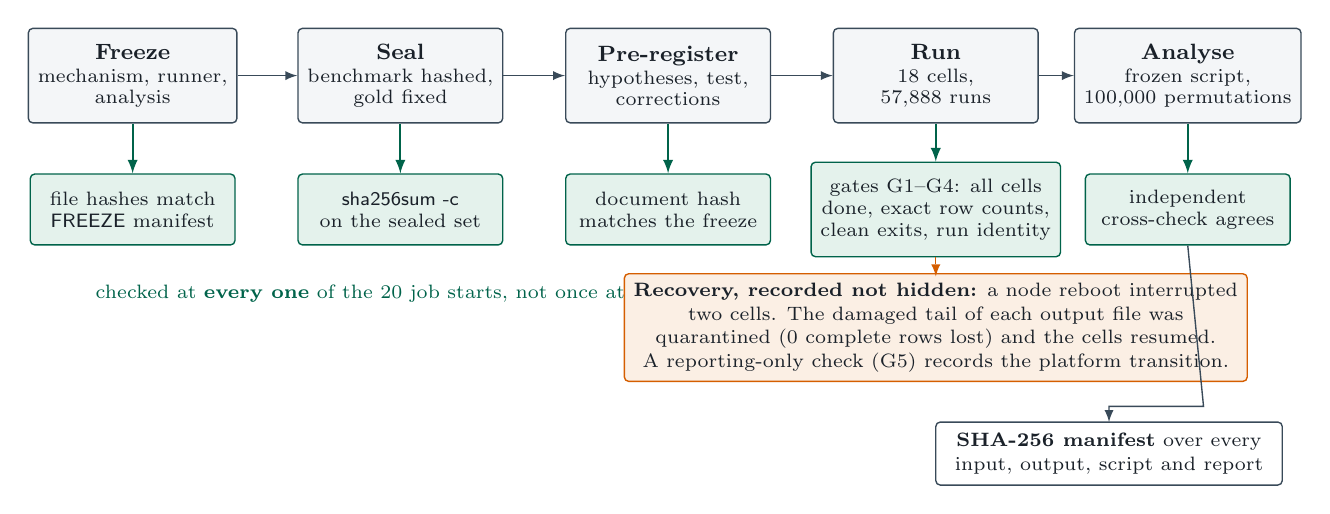
\begin{tikzpicture}[font=\footnotesize, x=1mm, y=1mm,
  stg/.style={blk, minimum width=26mm, minimum height=12mm, align=center},
  chk/.style={blkacc, minimum width=26mm, minimum height=9mm, align=center, font=\scriptsize}]

\node[stg] (freeze) at (16,34) {\textbf{Freeze}\\[-1pt]\scriptsize mechanism, runner,\\[-2pt]\scriptsize analysis};
\node[stg] (seal)   at (50,34) {\textbf{Seal}\\[-1pt]\scriptsize benchmark hashed,\\[-2pt]\scriptsize gold fixed};
\node[stg] (prereg) at (84,34) {\textbf{Pre-register}\\[-1pt]\scriptsize hypotheses, test,\\[-2pt]\scriptsize corrections};
\node[stg] (run)    at (118,34){\textbf{Run}\\[-1pt]\scriptsize 18 cells,\\[-2pt]\scriptsize 57{,}888 runs};
\node[stg] (anal)   at (150,34){\textbf{Analyse}\\[-1pt]\scriptsize frozen script,\\[-2pt]\scriptsize 100{,}000 permutations};

\foreach \a/\b in {freeze/seal, seal/prereg, prereg/run, run/anal} \draw[flow] (\a) -- (\b);

\node[chk] (c1) at (16,17) {file hashes match\\\cond{FREEZE} manifest};
\node[chk] (c2) at (50,17) {\cond{sha256sum -c}\\on the sealed set};
\node[chk] (c3) at (84,17) {document hash\\matches the freeze};
\node[chk, minimum height=12mm] (c4) at (118,17)
  {gates G1--G4: all cells\\done, exact row counts,\\clean exits, run identity};
\node[chk] (c5) at (150,17) {independent\\cross-check agrees};

\foreach \s/\c in {freeze/c1, seal/c2, prereg/c3, run/c4, anal/c5} \draw[flowacc] (\s) -- (\c);

\node[lbl, text=cEBG, anchor=north, align=center] at (50,8)
  {\scriptsize checked at \textbf{every one} of the 20 job starts, not once at the end};

\node[blkwarn, minimum width=54mm, minimum height=13mm, align=center] (recov) at (118,2)
  {\scriptsize \textbf{Recovery, recorded not hidden:} a node reboot interrupted\\[-1pt]
   \scriptsize two cells. The damaged tail of each output file was\\[-1pt]
   \scriptsize quarantined (0 complete rows lost) and the cells resumed.\\[-1pt]
   \scriptsize A reporting-only check (G5) records the platform transition.};
\draw[flowwarn] (c4.south) -- (118,8.5);

\node[blkplain, minimum width=44mm, minimum height=8mm, align=center] (man) at (140,-14)
  {\scriptsize \textbf{SHA-256 manifest} over every\\[-1pt]\scriptsize input, output, script and report};
\draw[flow] (c5.south) -- (152,-8) -- (140,-8) -- (140,-10);
\end{tikzpicture}

\vspace{1mm}
\caption[Experimental integrity chain]{%
\textbf{The integrity chain.} Each stage has a check that must pass before the next begins, and the checks on the
first three stages were re-run at every one of the 20 job starts rather than once at the end: all 20 reported zero
mechanism-file mismatches and the same pre-registration hash. The gates before analysis verify that all 18 cells
finished, that each holds exactly 268 $\times$ 12 unique (task, condition) pairs with no duplicate and no
unparsable line, that every cell's last job exited cleanly, and that the recorded run identity --- model, snapshot,
decoding, seed, dtype, parser, framework versions, and the hashes of all 14 mechanism files --- is identical across
every start of a cell. One deviation is recorded rather than smoothed over: an unplanned reboot interrupted two
cells, which resumed after the damaged tail of each file was quarantined, and a separate reporting-only check
documents the resulting platform transition (\Cref{sec:limitations}). Host names and addresses are deliberately
absent from this figure and from the released artifacts.\\
\emph{Accessible description:} a five-stage left-to-right chain, each stage with a check box beneath it, plus a
recovery note under the run stage and a final hash manifest.\\
\emph{Source:} \srcfile{PHASE3/scripts/finalize_gates.py}, \texttt{verify\_phase3.py},
\texttt{platform\_continuity.py}; \srcfile{PHASE3/PHASE3_SHA256_MANIFEST.txt}.}
\label{fig:integrity}
\end{figure}


\subsection{Provenance of every row}

Each cell writes a manifest at every start recording the model identity and resolved snapshot, the adapter (none
here) and its hash, decoding parameters and seed, dtype, maximum new tokens, parser version, family adapter,
framework and CUDA runtime versions, the GPU model, the split hash, the condition list, the SHA-256 of all 14
mechanism and harness files, the job id, the start time, and how many pairs were already complete at that start.
The 14 code hashes are identical across all 20 starts of the campaign. A SHA-256 manifest over every raw file is
written when the campaign closes and re-verified before anything is analysed (\Cref{fig:integrity}).

\subsection{Regenerating every number}

The whole pipeline runs as one CPU-only batch job with no interactive steps: integrity gates, staging, the
platform-continuity report, verification, the frozen analysis, the exploratory analyses, an independent
cross-check, report generation and a final hash manifest, stopping at the first failure. Every reported number
comes from that path; the independent cross-check must agree exactly or the pipeline stops, and the report
generator computes no statistic of its own. On the shareable development split the same pipeline reproduces its
outputs byte for byte.

\subsection{What a reproduction can and cannot match}

The \emph{analysis} is reproducible byte for byte from the archived raw outputs: permutations and bootstraps are
seeded and the gates re-verify the inputs first. Regenerating the \emph{raw outputs} is a weaker guarantee, with
three specific caveats: GPU kernels are not bitwise deterministic across hardware or library versions; two cells
were not produced on a single host platform and cannot be reproduced row for row on one driver version; and one of
those cells re-seeded its sampler when it resumed, so reproducing it byte for byte would require reproducing the
interruption at the same row (\Cref{tab:deviations}).

\subsection{Availability}

\textbf{Released with the paper:} the code (mechanism, harness, runner, analysis, integrity gates, tests), the
frozen manifests, the pre-registration, the development splits and their runs, all aggregate results in JSON and
CSV, the generated reports, the deviation ledger and the platform-continuity report, and a reproducibility package
documenting environment, model snapshots, dataset rules, batch scripts, analysis instructions, expected outputs,
tests, limitations and deviations, with SHA-256 manifests over all of it.

\textbf{Withheld until publication:} the eval3 items, their annotations and the per-run transcripts, so that the
test set stays uncontaminated; their hashes are public, so a later release can be checked against the frozen
versions. The cluster's per-run logs are withheld for the same reason, because their progress lines carry per-task
outcomes.

\textbf{Not redistributed:} model weights. The exact snapshot hashes are listed in the package; obtain the weights
under each model's own licence. Because the eval3 texts were written by Qwen2.5-14B-Instruct, that model's licence
terms on outputs apply to them.

Nothing here claims public availability for an artifact that is in fact restricted, and the released materials
contain no credentials, tokens, keys, host names, addresses or account identifiers; a check in the packaging
script fails the build if any appear.

\section{Conclusion and future work}
\label{sec:conclusion}

Small tool-using agents with persistent memory fail in a particular way when their records disagree: they follow a
reliability label instead of the text, and enforcing that label at the terminal action makes the failure worse.
This paper tested a specific alternative --- arbitration that states the \emph{evidence basis} for each resolution
and enforces only what that basis supports --- under a pre-registration frozen before the confirmatory data
existed.

The pre-registered result is positive and stable. Across 57{,}888 runs on 268 sealed tasks, gated evidence-basis
arbitration beat enforced record-and-temporal labels by $17.1$\pp{} of task success, advisory temporal labels by
$14.5$\pp, an LLM arbiter under the same policy by $15.9$\pp, and unlabelled memory by $15.3$\pp, all Holm
corrected, in the same direction for all six models and stable across three item-set definitions. Harmful answers
fell from 22.6\% to 3.1\%, and false resolution on genuinely unresolvable groups from 19.0\% to 1.9\%.

Three findings qualify what that means, and we regard them as the more useful part of the paper. Most of the gain
is in the labels, not the enforcement: evidence-basis labels alone are worth $11.8$\pp{} over metadata labels,
with gating adding $6.0$\pp. Ungated enforcement of those same labels scores $9.7$\pp{} higher still while doubling
harm and restoring the arbitrary picks the mechanism was built to prevent --- so gating trades accuracy for
safety, and this benchmark does not price that trade. And the same gating driven by an LLM arbiter produced no
gain and more harm, which suggests the general lesson is not about gating but about what enforcement is allowed to
enforce.

The best condition still answers only 61.3\% of tasks correctly, and its residual failure is over-conservatism:
20.2\% false conflicts and 11.5\% unnecessary abstentions against 3.1\% harm. The mechanism moved errors where it
was designed to move them. Whether that is the right place for them is a deployment judgement this study does not
make.

\paragraph{Future work.} Four directions follow directly. (1) A benchmark that assigns explicit costs to a wrong
confident answer and to a missed correct one, so that the gating trade can be decided rather than described.
(2) Extending the arbiter beyond lexical English cues and ISO value dates, where its documented limitations
currently live, and testing it on a set that excludes explicitly signalled invalidation
\citep{chao2026stale}. (3) A transcript study of the remaining false conflicts, to separate items the arbiter
could have resolved from items where abstaining is correct; this needs the data release. (4) Model-family
coverage: the Llama results show the mechanism helping by a different route, and a family whose dominant failure
is abstention needs a different account of what reliability means.

\paragraph{Two methodological artefacts} come out of the campaign rather than the results, and we release both.
Run manifests should record the host kernel, GPU driver and boot identifier, not only framework versions: in this
campaign a mid-campaign platform change was visible only as a 0.2\,GiB difference in a telemetry field. And an
integrity gate should separate what \emph{identifies} a run from what merely \emph{observes} its host, fail closed
on anything unclassified, and report the differences it is willing to tolerate rather than silently accepting or
silently rejecting them.


% long author-year labels can overflow their box; give the bibliography extra breaking freedom
\begingroup
\sloppy
\emergencystretch=4em
\bibliographystyle{tmlr}
\bibliography{references}
\endgroup

\appendix
\section{Pre-registered verdict rules}
\label{app:verdicts}

The verdict for each hypothesis was fixed before the data existed and applied mechanically by the analysis script.
For H-primary and S1--S3 a hypothesis is \emph{supported} if its Holm-adjusted $p<0.05$ \emph{and} its 95\%
confidence interval lies entirely above zero; otherwise it is \emph{not supported}. S4 has only two possible
verdicts: it is \emph{falsified} if the confidence interval for the \cond{EBG} $-$ \cond{RT} harmful difference
lies entirely above zero, or if \cond{EBG}'s arbitrary-pick count exceeds \cond{RT}'s; otherwise it is \emph{not
falsified}. No verdict rule was changed after the freeze, and the script that applies them is released.

\section{Condition-level rates}
\label{app:rates}

\Cref{tab:rates} gives the pooled primary rates behind \Cref{fig:tradeoff} and \Cref{fig:failures}. Per-model
tables, per-decoding tables, per-category tables and the full set of contrasts for every item set are in the
supplementary material.

\begin{table}[h]
\centering
\caption{Outcome rates by condition, pooled over the four primary models and four decodings ($n=4288$ runs per
condition). Conflict preservation and false resolution are over conflict groups and are pooled over all six
models. Source: \srcfile{PHASE3/results/per_model_config.csv} and
\srcfile{PHASE3/ANALYSIS/METRICS.json}.}
\label{tab:rates}
\small
\setlength{\tabcolsep}{4.4pt}
\begin{tabular}{@{}lrrrrrrr@{}}
\toprule
\textbf{Cond.} & \textbf{Success} & \textbf{Harmful} & \textbf{Arb.} & \textbf{Unnec.} & \textbf{Format} & \textbf{Conflict} & \textbf{False} \\
 & \% & \% & \textbf{picks} & \textbf{abst.\ \%} & \textbf{err.\ \%} & \textbf{pres.\ \%} & \textbf{res.\ \%} \\
\midrule
\cond{B}           & 46.0 & 7.0  & 172 & 19.5 & 3.2 & 65.2 & 12.8 \\
\cond{G}           & 43.5 & 7.9  & 109 & 16.0 & 3.7 & 72.8 & 9.2  \\
\cond{T}           & 46.9 & 7.4  & 35  & 16.9 & 3.1 & 79.6 & 3.6  \\
\cond{R}           & 45.0 & 16.1 & 153 & 9.4  & 6.1 & 74.2 & 12.3 \\
\cond{RT}          & 44.2 & 22.6 & 252 & 11.1 & 6.2 & 66.8 & 19.0 \\
\cond{LA}          & 47.9 & 13.2 & 295 & 18.4 & 3.5 & 57.8 & 21.9 \\
\cond{LG}          & 45.4 & 21.3 & 510 & 17.1 & 3.3 & 42.4 & 37.0 \\
\cond{EB}          & 55.3 & 2.7  & 13  & 16.7 & 3.1 & 81.6 & 2.0  \\
\textbf{\cond{EBG}} & \bfseries 61.3 & \bfseries 3.1 & \textbf{13} & \bfseries 12.8 & \bfseries 3.3 & \bfseries 88.5 & \bfseries 1.9 \\
\cond{EBG-all}     & 71.1 & 6.9  & 166 & 13.9 & 3.3 & 77.3 & 12.9 \\
\cond{EBG-unsafe}  & 61.5 & 3.3  & 12  & 9.9  & 6.4 & 89.0 & 1.6  \\
\cond{EBG-noR3}    & 60.0 & 3.4  & 14  & 17.6 & 2.9 & 83.3 & 1.9  \\
\bottomrule
\end{tabular}
\end{table}

\section{Supplementary material}
\label{app:supp}

The supplement contains the full per-model and per-decoding result tables, the complete contrast set for all four
item sets, the extended failure tables, the detailed benchmark construction and annotation protocol, the
deviation ledger with its evidence classified as verified, inferred or unknown, and the reproduction instructions.
It contains no eval3 task text, gold label, per-run transcript, credential or infrastructure identifier.


\end{document}
